\chapter*{第一部分:总论}
\markboth{总论}{总论}

\begin{figure}[htbp]
	\centering
	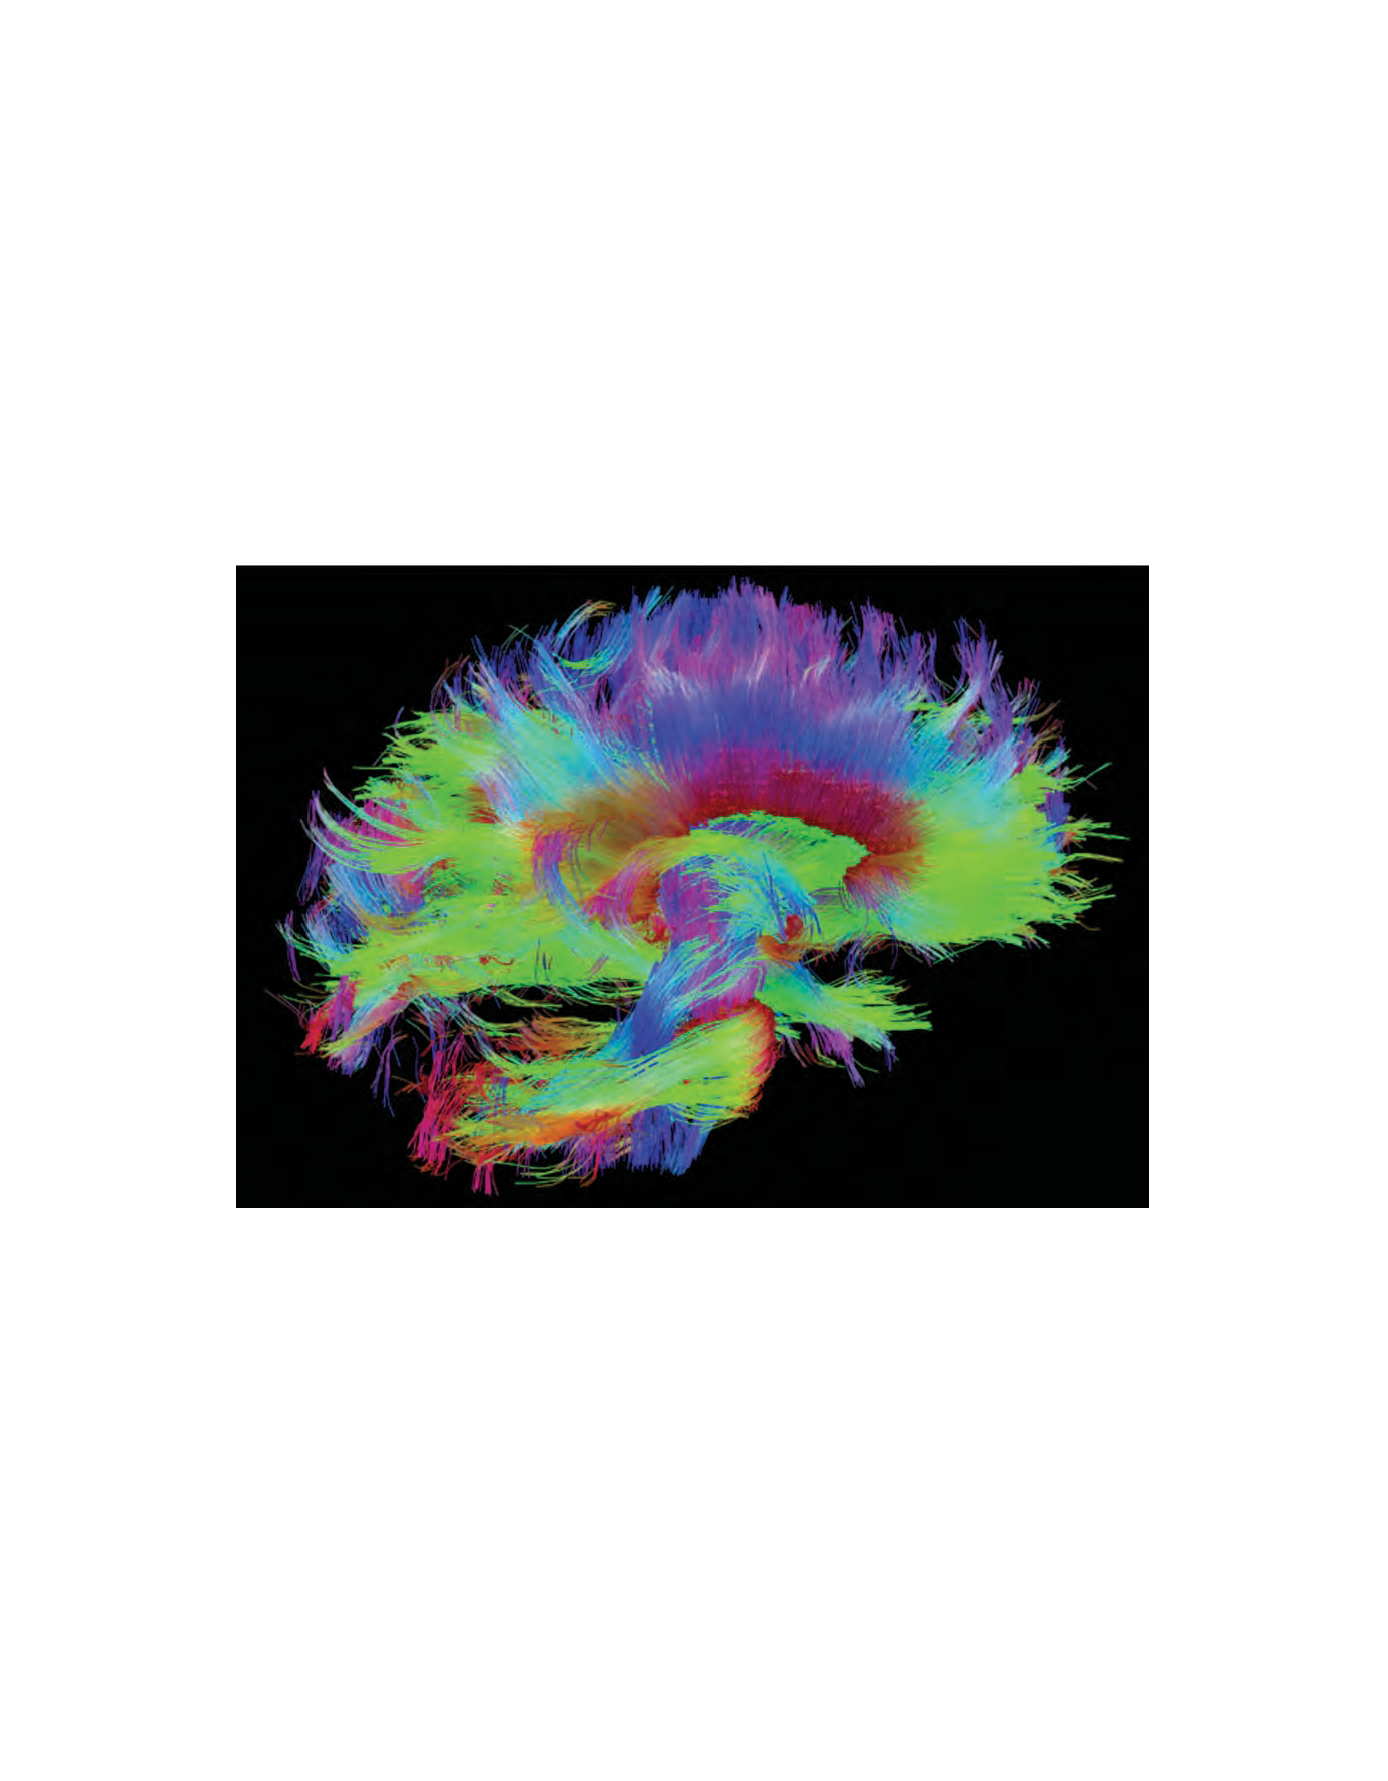
\includegraphics[width=1.0\linewidth]{chap01/fig_1_0}
	\caption{人脑白质纤维结构,显示胼胝体和脑干通路。
		该图像是根据\textit{核磁共振成像}数据和扩散光谱成像技术构建的,该技术使用水分子的扩散速率和优选方向在核磁共振图像中产生对比度,以揭示在纤维束中行进的轴突束。
		纤维按方向进行颜色编码:红色,左右;绿色,前后;蓝色,升序-降序(RGB=XYZ轴)。
		(来自连接体扫描仪数据集。
		由南加州大学神经成像实验室和哈佛大学生物医学成像中心提供。
		\href{www.humanconnetomproject.org}{人类连接体项目联合会})}
	\label{fig:1_0}
\end{figure}

在20世纪下半叶,生物学的中心焦点是基因。
现在,在21世纪上半叶,焦点已经转移到神经科学,特别是\textit{心理生物学}。
我们希望了解我们感知、行动、学习和记忆的过程。
一个只有 1.5 公斤重的大脑器官是如何构思无限、发现新知识并产生人类思想、情感和行动的非凡个性?
这些非凡的心理能力是如何在器官内分布的?
什么规则将一个区域的解剖组织和细胞生理与其在心理状态中的特定作用联系起来?
基因对行为有什么影响?
神经细胞中的基因表达是如何受到发育和学习过程的调节?
经验是如何改变大脑处理后续事件的方式,以及这种处理在多大程度上是无意识的?
最后,神经和精神疾病的神经基础是什么?
在《神经科学原理》的介绍部分,我们开始讨论这些问题。
在这样做的过程中,我们描述了神经科学如何试图将神经回路的计算逻辑与大脑联系起来,即定义的神经回路中的神经细胞活动如何介导复杂的心理过程。


在过去的几十年里,技术进步为大脑的科学研究开辟了新的视野。
今天,有可能将神经元互连回路的细胞动力学与大脑中感知和运动行为的内部表征联系起来,并将这些内部机制与可观察的行为联系起来。
新的成像技术使我们能够可视化人类大脑的活动,即识别大脑中与特定思维和感觉模式及其相互联系模式相关的特定区域。


在本书的第一部分中,我们考虑了心理功能在多大程度上可以定位到大脑的特定区域。
我们还研究了这些功能在多大程度上可以从单个神经细胞的特性、它们的分子成分突触连接来理解。
在本书的后面部分,我们详细研究了大脑认知和情感功能的基本机制:感知、行动、动机、情绪、学习和记忆。


人脑是一个由 800 多亿个神经细胞组成的网络,这些神经细胞在系统中相互连接(神经回路)构建我们对外部世界的感知,固定我们的注意力,指导我们的决策,并实施我们的行动。
因此,理解大脑的第一步是了解神经元是如何组织成信号通路的,以及它们是如何通过突触传递进行交流的。
我们将在本书中提出的主要观点之一是,在\textit{发育过程中建立}并在\textit{经验过程中完善}的\textit{突触连接特异性}是行为的基础。
我们还必须了解行为的先天和环境决定因素,在这些决定因素中,基因编码的蛋白质最初控制着神经回路的发育,然后可以通过基因表达的经验依赖性变化来改变神经回路。


通过将现代细胞和分子生物学技术、大脑成像、理论和临床观察应用于认知、情绪和行为的研究,一门新的心理科学正在兴起。
神经科学强化了希波克拉底在两千多年前首次提出的观点,即对心智的正确研究始于对大脑的研究。
认知心理学和精神分析理论强调了人类心理体验的多样性和复杂性。
这些学科现在可以通过从神经科学中深入了解大脑功能来丰富。
未来的任务是对心理过程进行研究,以实证神经科学为基础,关注心理的内部表征和状态是如何产生的问题。


我们的目标不仅仅是提供事实,而是提供大脑组织、功能和计算的原理。
神经科学原理并没有将人类思想的复杂性简化为一组分子或数学公理。
相反,它们让我们能够在大脑的复杂性中欣赏到某种美,即达尔文式的优雅,这种复杂性解释了思维和行为。
人们可能会问,从更基本的神经机制的详细解剖中收集到的一个想法是否包含了对更高大脑功能的见解。
简单反射的组织是否与手的意志运动有关?
在发育中的脊髓中建立回路的机制是否与存储记忆的机制有关?
将我们从睡眠中唤醒的神经过程与允许无意识过程刺穿我们意识的过程相似吗?
我们希望读者在深入研究其事实基础时,会对这些原则感到高兴。
毫无疑问,这是一项正在进行的工作。





\chapter{大脑和行为} \label{chap:chap1}
生物科学的最后前沿(终极挑战)是理解意识的生物学基础和我们感知、行为、学习和记忆的大脑过程。 
在过去的几十年里,生物科学内部的显著统一为应对这一巨大挑战奠定了基础。 
对基因进行测序并推断它们编码蛋白质的氨基酸序列揭示了神经系统中的蛋白质与身体其他部位的蛋白质之间意想不到的相似性。 
因此,建立细胞功能的总体计划成为可能,该计划为包括细胞神经科学在内的所有细胞生物学提供了一个共同的概念框架。


当前生物学统一的挑战是心理学、心智科学、神经科学和大脑科学的统一。 
在这种统一的方法中,不将思想和身体视为独立的实体,基于这样一种观点,即所有行为都是大脑功能的结果。 
我们通常所说的心智是由大脑执行的一系列操作。 
大脑过程不仅是行走和进食等简单运动行为的基础,也是典型人类的所有复杂认知和行为的基础,即思考、说话和创作艺术作品。 
作为推论,所有表征精神疾病的行为障碍(感觉上的情感障碍和思想上的认知障碍)都是脑功能紊乱的结果。


大脑中数十亿个神经细胞如何产生行为和认知状态,以及这些细胞如何受到环境(包括社会经验)的影响? 
用大脑活动来解释行为是神经科学的重要任务,神经科学在这方面的进展是本书的一大主题。


神经科学必须不断面对某些基本问题。 
理解思维过程、肢体运动或做出运动愿望的适当生物学描述水平是多少? 
为什么在某些神经系统疾病状态下运动会平稳或急促或无意中进行? 
通过观察神经细胞中\textit{脱氧核糖核酸}表达的模式以及这种模式如何调节神经元的电特性,可能会得出这些问题的答案。 
然而,我们还需要了解由特定大脑区域中的许多神经元组成的神经回路以及许多大脑区域中特定回路的活动如何协调的知识。


是否存在最恰当的生物学描述水平?
简短的回答是,
如果一个人的目标是了解和治疗某些遗传性癫痫病症,那么\textit{脱氧核糖核酸}测序和单个神经元电特性的测量可能足以产生有效的治疗方法。
如果一个人对学习、感知和探索感兴趣,那么可能需要对回路系统和大脑区域进行分析。


现代神经科学的目标是将所有这些专业水平整合成一门连贯的科学。
这种努力迫使我们面对新的问题。
如果心理过程可以定位到离散的大脑区域,那么这些区域的功能与这些区域的解剖学和生理学之间的关系是什么? 
是否需要一种神经回路来处理视觉信息,另一种神经回路来解析语音,还有另一种神经回路来排列运动?
或者具有不同功能的回路是否具有共同的组织原则?
必要的神经计算是否最好理解为对单个神经元或神经元群表示的信息的操作?
信息是以单个神经细胞的电活动表示的,还是分布在整体上的,以至于任何一个细胞的信息量都不比计算机内存的随机位多?
正如我们将要看到的,关于组织水平、细胞特化和功能定位的问题在整个神经科学中反复出现。


为了说明这些观点,我们将研究现代神经科学如何描述语言,这是人类独特的认知行为。
这样做将广泛关注大脑皮层的运作,大脑皮层是人类大脑中最发达的部分。
将看到大脑皮层如何组织成功能不同的区域,每个区域由许多神经元组成,以及如何根据特定区域内特定组互连神经元的活动来分析高度复杂行为的神经装置。
第~\ref{chap:chap3}~章描述了简单反射行为的神经回路如何在细胞水平上运作,说明了感觉信号和运动信号的相互作用如何导致运动行为。



% 结构(几何)和功能(行为)
\section{关于大脑与行为之间的关系,提出了两种相反的观点}

关于神经细胞、大脑和行为的观点是在 20 世纪从 5 种实验传统的综合中产生的:解剖学、胚胎学、生理学、药理学和心理学。


公元 2 世纪的希腊医生盖伦提出,神经将大脑和脊髓分泌的液体输送到身体的周围。
他的观点主导了西方医学,直到显微镜揭示了神经组织中细胞的真实结构。
即便如此,直到 19 世纪后期,神经组织才成为一门特殊科学的主题,当时意大利人\textit{卡米洛$\cdot$高尔基}和西班牙人圣地\textit{亚哥$\cdot$拉蒙$\cdot$卡哈尔}对神经细胞进行了详细、准确的描述,但就大脑的功能得出了两个截然不同的结论。


高尔基开发了一种用银盐对神经元进行染色的方法,这种方法可以在显微镜下显示出它们的整个细胞结构。
基于这些研究,高尔基体得出结论,神经细胞不是相互隔离的独立细胞,而是在一个连续的组织或合胞体网络中共同作用。
使用高尔基技术,\textit{卡哈尔}扩观察到每个神经元通常都有一个细胞体和两种类型的过程:一端是分支树突,另一端是长长的电缆状轴突。 
\textit{卡哈尔}扩得出结论,神经组织不是合胞体,而是离散细胞网络。
在这项工作的过程中,\textit{卡哈尔}扩发展了神经元学说的一些关键概念和许多早期证据,即个体神经元是神经系统的基本构建块和信号元件的原则。


在 1920 年,美国胚胎学家\textit{罗斯$\cdot$哈里逊}表明树突和轴突是从细胞体中生长出来的,即使在组织培养中每个神经元都与其他神经元隔离开来也是如此。
\textit{哈里逊}还证实了\textit{卡哈尔}的提议,即轴突的尖端会产生扩张,即生长锥,它将发育中的轴突引导至其目标,即其他神经细胞或肌肉。
这两项发现都为神经元学说提供了强有力的支持。
随着电子显微镜的引入,神经元学说的最终明确证据出现在 20 世纪 50 年代中期。
\textit{桑福德$\cdot$帕莱}的一项具有里程碑意义的研究明确地证明了突触的存在,突触是神经细胞的特殊区域,允许它们之间进行化学或电信号传递。


神经系统的生理学研究始于 18 世纪后期,当时意大利医师和物理学\textit{路易吉$\cdot$加尔瓦尼}发现肌肉和神经细胞会产生电能。
现代电生理学起源于 19 世纪三位德国生理学家:\textit{约翰内斯$\cdot$米勒}、\textit{埃米尔$\cdot$杜$\cdot$博伊斯-雷蒙德}和\textit{赫尔曼$\cdot$冯$\cdot$亥姆霍兹},他们成功地测量了电活动沿神经细胞轴突的传导速度,并进一步表明:
一个神经细胞的电活动以可预测的方式影响相邻细胞的活动。


药理学在 19 世纪末对我们对神经系统和行为的理解产生了第一次影响,当时法国的\textit{克劳德$\cdot$伯纳德}、德国的\textit{保罗$\cdot$埃尔利希}和英国的\textit{约翰$\cdot$兰利}证明药物不会随机作用于细胞,而是通常与位于细胞膜中的离散受体结合。 
这种洞察力导致发现神经细胞可以通过化学方式相互交流。


关于行为的心理学思考可以追溯到西方科学的开端,当时古希腊哲学家推测行为的原因以及心灵与大脑的关系。
在随后的几个世纪里,出现了两种主要观点。
在 17 世纪,笛卡尔区分了身体和心灵。
在这种二元论观点中,大脑调解了知觉、运动行为、记忆、食欲和激情,即一切可以在低等动物身上找到的东西。
但是心智(更高的心智功能,人类行为的有意识体验特征)并不代表大脑或身体的任何其他部分,而是代表灵魂,一个精神实体。
笛卡尔认为,灵魂通过松果体与大脑的机器进行交流,松果体是大脑中线的一个微小结构。
笛卡尔的立场在现代哲学或神经科学中几乎没有影响力。
事实上,神经科学的基本前提是心智是大脑及其神经活动的产物。
我们这样说并不是说神经科学的目的是通过还原为生物成分来解释心灵,而是要阐明心灵的生物学。


早在 1800 年,维也纳医生和神经解剖学家\textit{弗朗兹$\cdot$约瑟夫$\cdot$加尔}就开始尝试将生物学和心理学概念结合到行为研究中,当时他提出了一种全新的身心观念。
他主张大脑是心灵的器官,一切精神功能都体现在大脑中。
因此,他拒绝了笛卡尔认为思想和身体是分开实体的观点。
此外,他认为大脑皮层不是一个单一的器官,而是包含许多专门的器官,大脑皮层的特定区域控制着特定的功能。 
\textit{加尔}列举了至少 27 个不同的大脑皮层区域或器官; 后来又增加了更多,每一种都对应于一种特定的心智能力(图~\ref{fig:1_1})。
\textit{加尔}将智力过程(例如评估因果关系、计算和感知秩序的能力)分配给了大脑的前部。
浪漫的爱情(恋爱)和好斗的本能特征被分配到大脑后部。
即使是最抽象的人类行为(慷慨、隐秘和虔诚)也被分配到大脑中的一个位置。


\begin{figure}[htbp]
	\centering
	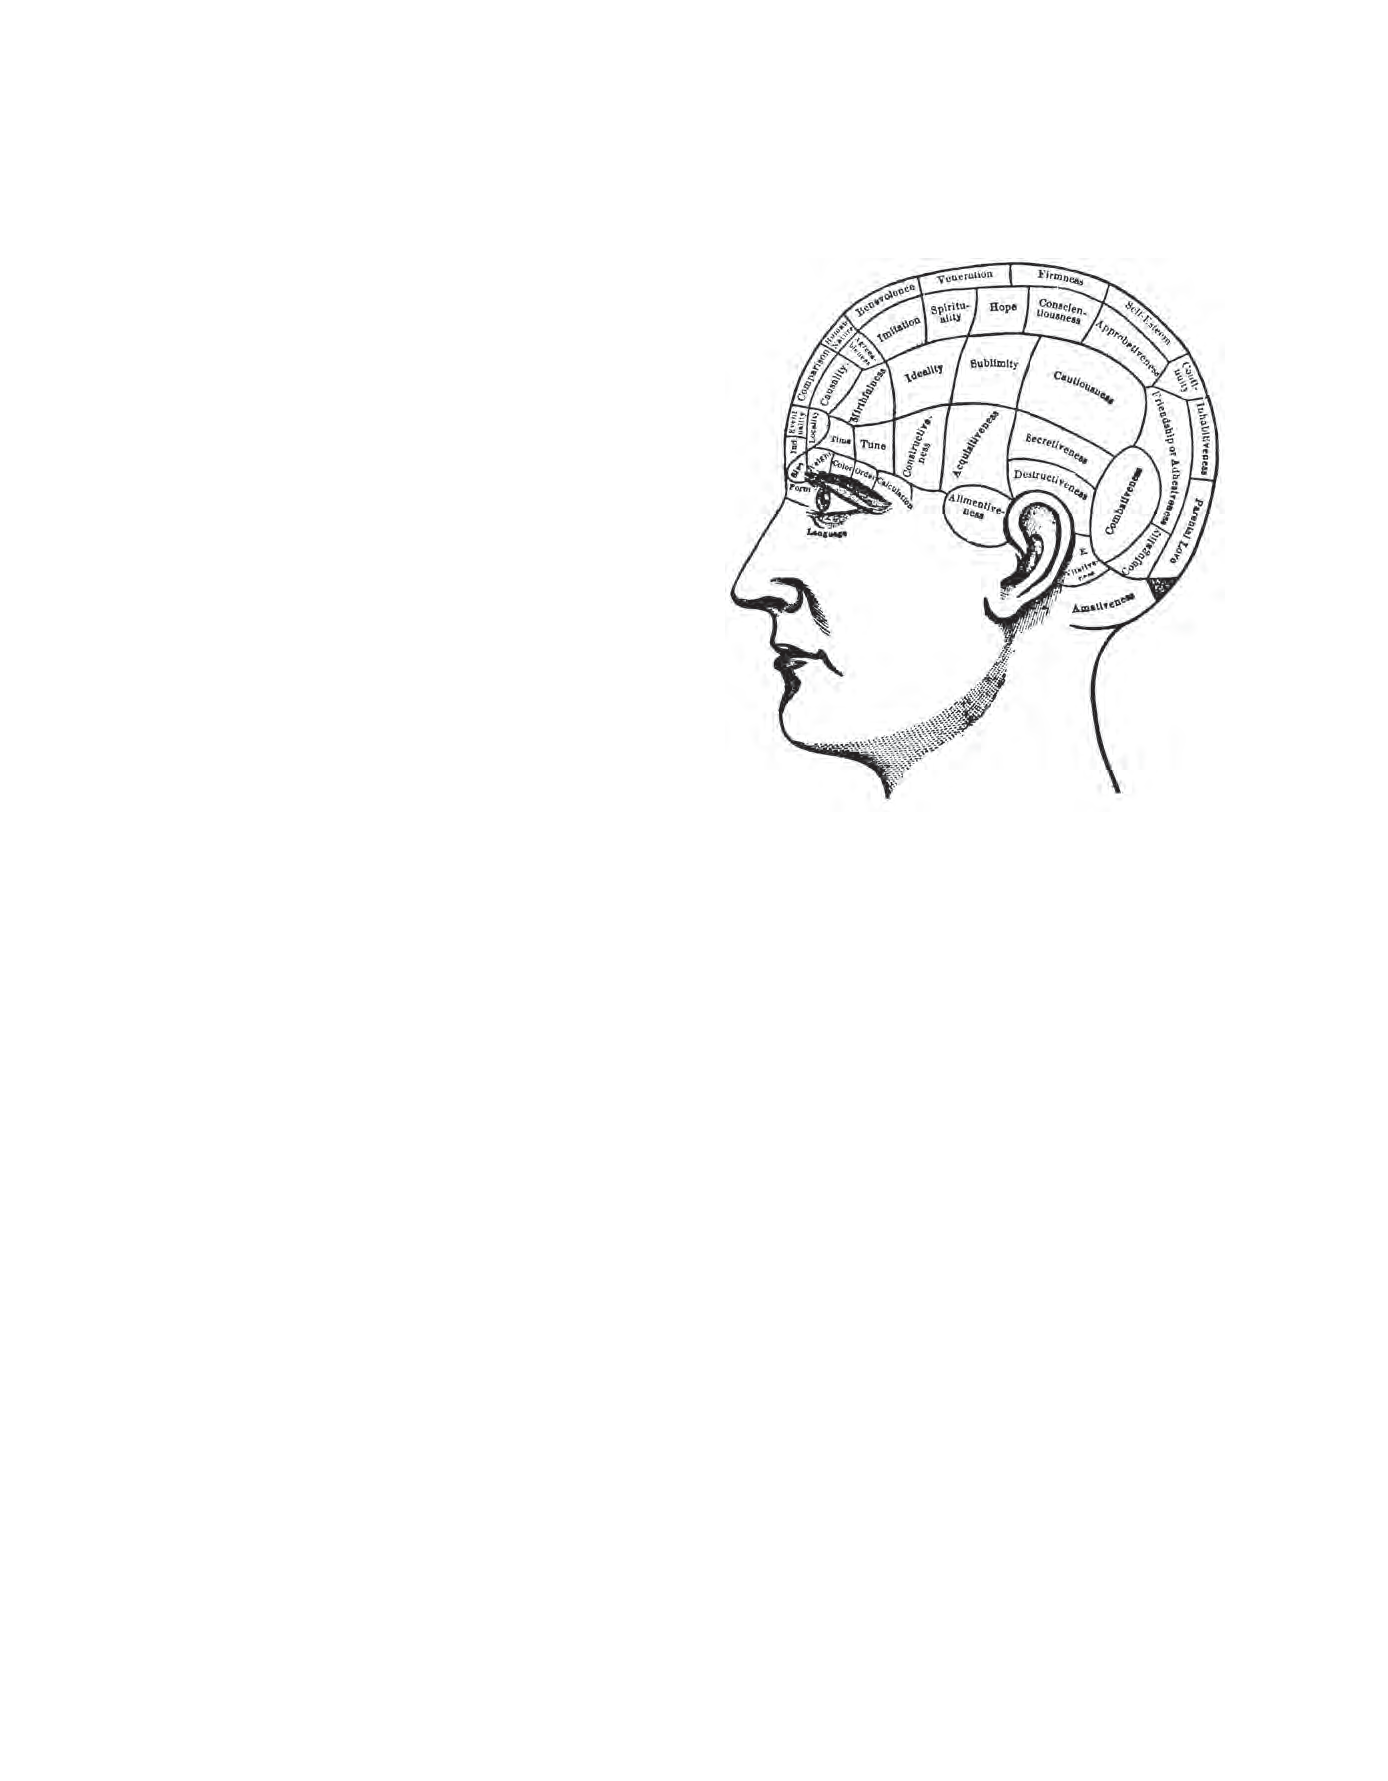
\includegraphics[width=0.55\linewidth]{chap01/fig_1_1}
	\caption{大脑功能定位的早期地图。
		根据 19 世纪的颅相学学说,好斗、灵性、希望和责任心等复杂特征由专门的“器官”控制,大脑皮层的不同区域随着特征的发展而扩大。
		这些大脑局部区域的扩大被认为会在覆盖的头骨上产生特征性的凹凸,从中可以确定一个人的性格。
		这张地图取自 1800 年代初期的一幅图画,显示了 42 个智力和情感“器官”。}
	\label{fig:1_1}
\end{figure}


尽管\textit{加尔}的身心统一理论和他关于某些功能局限于特定大脑区域的观点被证明是正确的,但今天的主流观点是,许多高层心理功能很可能是高度分布的。
此外,\textit{加尔}的本地化实验方法极其幼稚。
\textit{加尔}没有根据经验定位功能,而是通过研究大脑并将心理属性的缺陷与肿瘤或中风后特定区域的病变相关联,\textit{加尔}摒弃了所有来自脑部病变研究的证据,无论是通过临床检查发现的还是在实验动物身上通过手术产生的。
受\textit{相面术}的影响,这是一门基于面部特征揭示性格的流行科学,\textit{加尔}认为,具有特定认知能力的人头骨上的隆起和隆起确定了大脑中这些能力的中心。
他假设大脑区域的大小与该区域所代表的心智能力的相对重要性有关。
因此,特定智力的锻炼会导致相应的大脑区域生长,而这种生长又会导致覆盖在上面的头骨突出。


小时候,\textit{加尔}注意到他那些擅长背作业的同学都有突出的眼睛,于是他就有了这个想法。
他得出结论,这是大脑前部与语言记忆有关的区域过度发育的结果。
当他还是一名年轻医生时,他进一步发展了这个想法,负责管理维也纳的一家精神病院。
在那里,他开始研究患有偏执狂症的患者,这种疾病的特征是对某些关键思想过分感兴趣或强烈渴望从事某些特定行为,比如盗窃、谋杀、色情、极端宗教信仰。
他推断,由于患者在所有其他行为中都表现良好,大脑缺陷一定是离散的,原则上可以通过检查这些患者的头骨来定位。
\textit{加尔}对局部大脑功能的研究催生了颅相学,这是一门根据头骨的详细形状确定人格和性格的学科。


在 1820 年代后期,法国生理学家\textit{皮埃尔$\cdot$弗卢龙}对\textit{加尔}的想法进行了实验分析。 
\textit{弗卢龙}使用实验动物破坏了\textit{加尔}在大脑中的一些功能中心,进而试图分离出这些“大脑器官”对行为的贡献。
从这些实验中,\textit{弗卢龙}得出结论,特定的大脑区域并不负责特定的行为,而是所有的大脑区域,尤其是前脑的大脑半球,都参与了每一次心理操作。
\textit{弗卢龙}提出,大脑半球的任何部分都有助于半球的所有功能。
因此,大脑半球任何一个区域的损伤都应该平等地影响所有更高的功能。
因此,在 1823 年,\textit{弗卢龙}写道:“所有知觉、所有意志都在这些(大脑)器官中占据相同的位置;
因此,知觉、构想和意志的能力仅仅构成了一种本质上是一体的能力。”


这种信念的迅速接受,后来被称为大脑的整体观点,仅部分基于\textit{弗卢龙}的实验工作。
它也代表了对人类思想是生物器官的唯物主义观点的文化反应。
它代表了对没有灵魂、所有心理过程都可以简化为大脑内的活动以及可以通过锻炼来改善思想的观念的拒绝,这些想法是欧洲宗教机构和土地贵族所不能接受的。


然而,在 19 世纪中叶,法国神经学家\textit{皮埃尔$\cdot$保尔$\cdot$布罗卡}、德国神经学家\textit{卡尔$\cdot$韦尼克}和英国神经学家\textit{休林斯$\cdot$杰克逊}严重挑战了整体观点。
例如,杰克逊在他对局灶性癫痫(一种以身体特定部位开始抽搐为特征的疾病)的研究中表明,不同的运动和感觉功能可以追溯到大脑皮层的特定部位。
\textit{布洛卡}、\textit{韦尼克} 和\textit{杰克逊}的区域研究被 \textit{查尔斯$\cdot$谢灵顿}和\textit{卡哈尔}扩展到细胞水平,他们支持称为细胞连接主义的大脑功能观点。
根据这种观点,单个神经元是大脑的信号单元;
它们按功能组排列,并以精确的方式相互连接。
\textit{韦尼克}和法国神经学家\textit{朱尔斯$\cdot$代热林}的研究表明,不同的行为是由不同的相互关联的大脑区域产生的。


本地化的第一个重要证据来自对大脑如何产生语言的研究。
在考虑相关的临床和解剖学研究之前,首先要回顾一下大脑的整体结构,包括它的主要解剖区域。
这需要我们定义一些神经解剖学家用来描述大脑和脊髓部分之间三维空间关系的基本导航术语。
这些术语在框~\ref{box:1_1}~和图~\ref{fig:1_2}~中介绍。


\begin{proposition}[神经解剖学导航术语] \label{box:1_1}
	
	\quad \quad 中枢神经系统各组成部分在体内的位置和方向参照三个轴进行描述:嘴侧-尾侧、背侧-腹侧和内侧-外侧轴(图~\ref{fig:1_2})。
	这些术语使神经解剖学家能够描述大脑和脊髓部分之间的空间关系。
	它们有助于在同一物种的个体发育或疾病情况下对其大脑进行比较。
	例如,它们也有助于比较不同动物物种的大脑,以了解大脑的进化。

\end{proposition}


\begin{figure}[htbp]
	\centering
	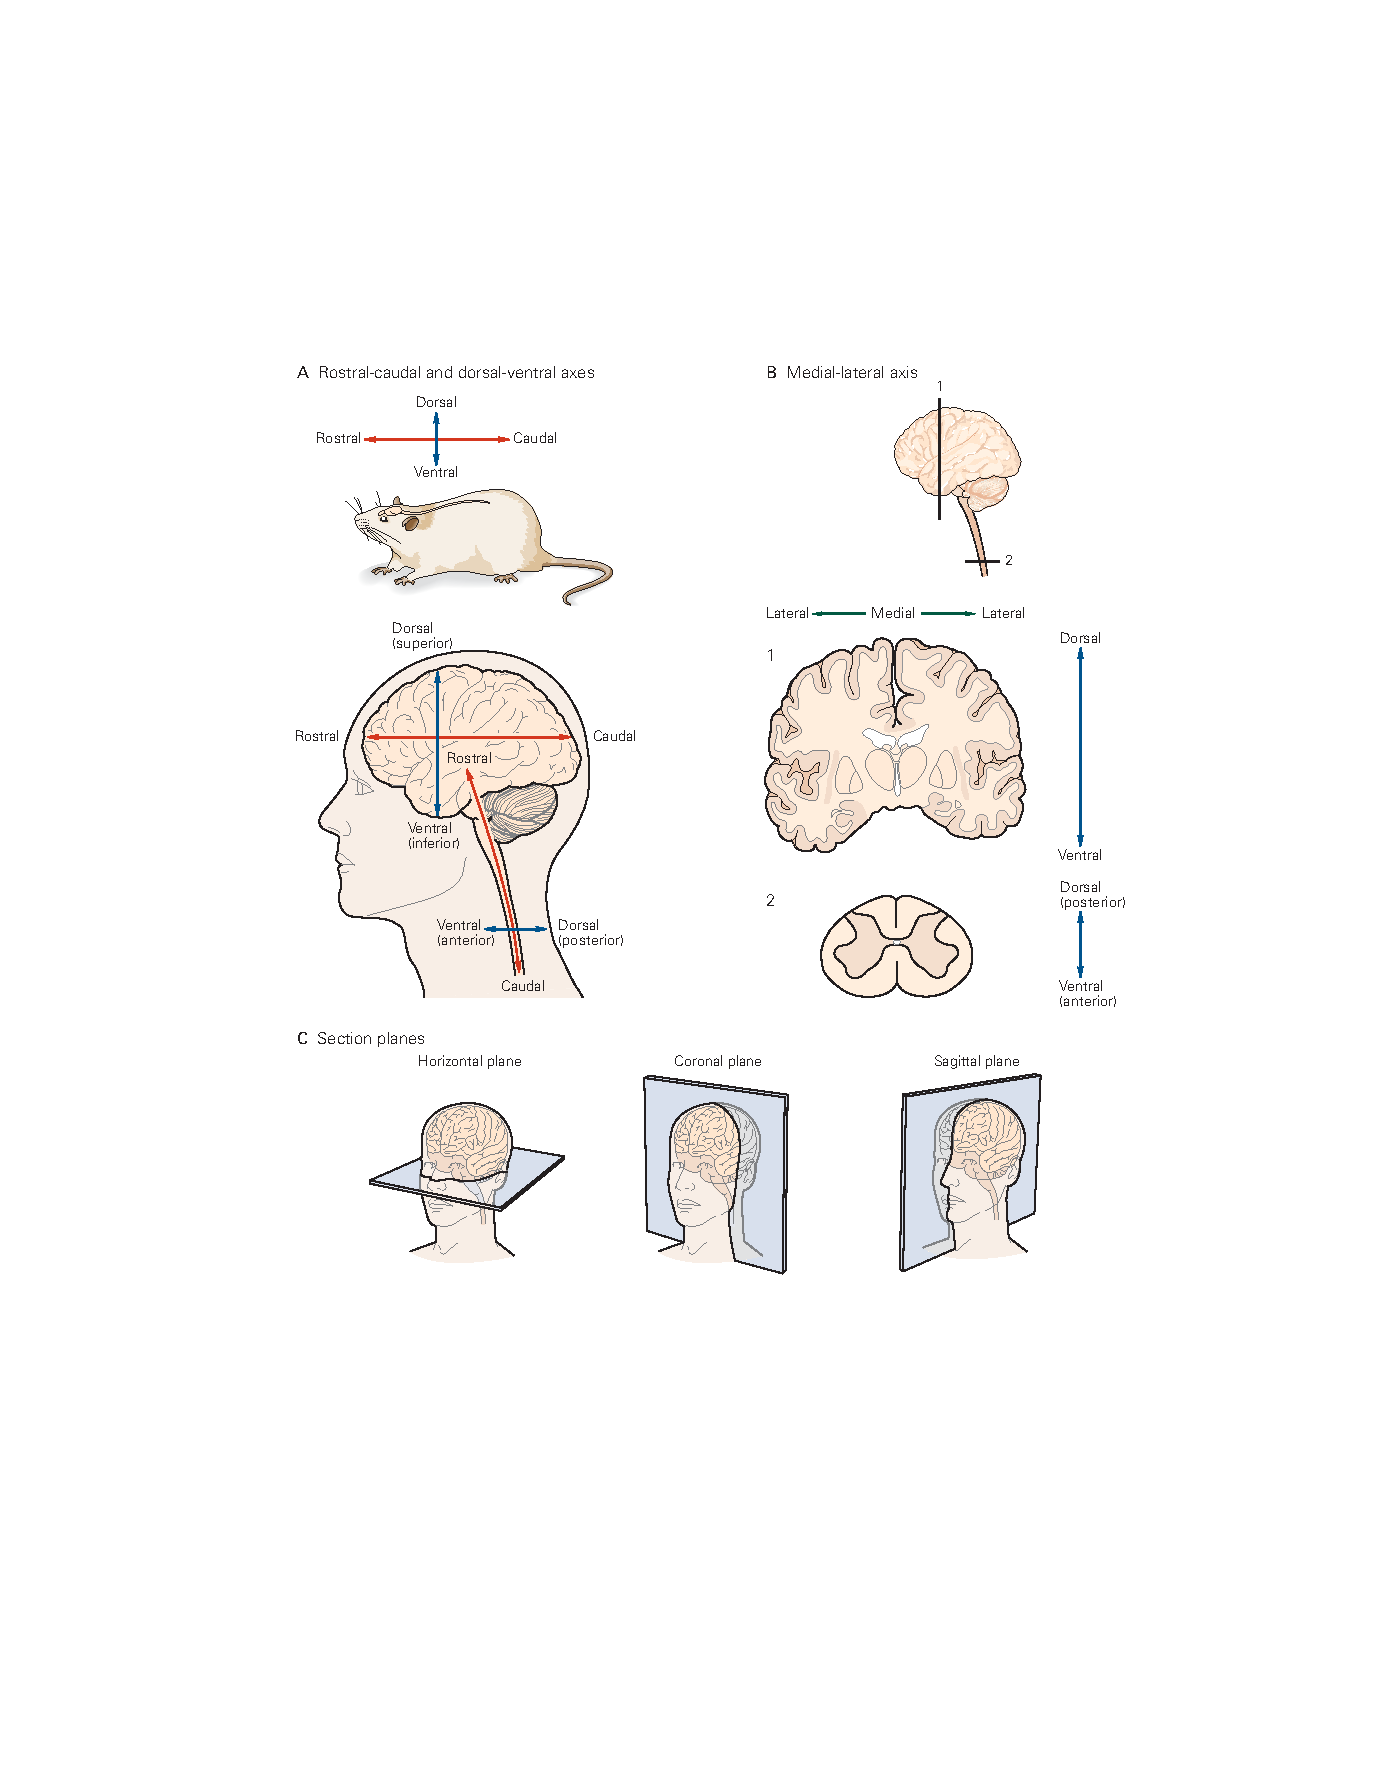
\includegraphics[width=0.95\linewidth]{chap01/fig_1_2}
	\caption{中枢神经系统沿着三个主要轴进行描述\cite{martin2012neuroanatomy}。 
		\textbf{A.} 嘴侧表示朝向鼻子和尾部朝向尾巴。
		背侧是指朝向动物的背部,腹侧是指朝向腹部。
		在低等哺乳动物中,这两个轴的方向在发育到成年生活的过程中一直保持不变。
		在人类和其他高等灵长类动物中,纵轴在脑干中弯曲大约 110 度。
		由于这种挠曲,相同的位置术语在指代挠曲下方和上方的结构时具有不同的含义。
		在弯曲下方,在脊髓中,嘴侧意味着朝向头部,尾侧意味着朝向尾骨(脊柱的下端),腹侧(前侧)意味着朝向腹部,背侧(后侧)意味着朝向背部。
		在弯曲上方,嘴侧意味着朝向鼻子,尾侧意味着朝向后脑勺,腹侧意味着朝向下巴,背侧意味着朝向头顶。
		术语上位通常与背侧同义,下位与腹侧相同。
		\textbf{B.} 内侧意味着朝向大脑中部,外侧意味着朝向侧面。
		\textbf{C.} 当对大脑进行切片进行分析时,切片通常是在三个基本平面之一中制作的:水平、冠状或矢状。}
	\label{fig:1_2}
\end{figure}



\section{大脑具有不同的功能区域}

中枢神经系统是一个双侧且基本对称的结构,有两个主要部分,即脊髓和大脑。
大脑包括六个主要结构:延髓、脑桥、小脑、中脑、间脑和大脑(方框~\ref{box:1_2}~和图~\ref{fig:1_3})。
这些中的每一个依次包含具有独特连接性和发育起源的不同神经元组。
在延髓、脑桥、中脑和间脑中,神经元通常分为不同的簇,称为细胞核。
大脑和小脑的表面由一大片折叠的神经元组成,分别称为大脑皮层和小脑皮层,其中神经元以固定的连接模式分层组织。
大脑还包含许多位于皮层(皮层下)下方的结构,包括基底神经节和杏仁核(图~\ref{fig:1_4})。


\begin{proposition}[中枢神经系统的解剖学组织] \label{box:1_2}
	\textbf{中枢神经系统有七个主要部分}
	
	\quad \quad \textbf{脊髓}是中枢神经系统的最尾部,接收和处理来自四肢和躯干皮肤、关节和肌肉的感觉信息,并控制四肢和躯干的运动。
	如图~\ref{fig:1_3}~所示,它被细分为颈部、胸部、腰部和骶骨区域。
	
	\quad \quad 脊髓继续作为\textbf{脑干}向头端延伸,脑干由延髓、脑桥和中脑组成。
	脑干接收来自头部皮肤和肌肉的感觉信息,并为头部肌肉组织提供运动控制。
	它还将信息从脊髓传递到大脑,从大脑传递到脊髓,并通过网状结构调节唤醒和意识水平。
	
	\quad \quad 脑干包含几个细胞体集合,即脑神经核。
	其中一些细胞核接收来自头部皮肤和肌肉的信息;
	其他人控制面部、颈部和眼睛肌肉的运动输出。
	还有一些人专门处理来自三种特殊感官的信息:听觉、平衡和味觉。
	
	\quad \quad \textbf{延髓}直接位于脊髓的嘴侧,包括几个负责重要自主功能的中心,如消化、呼吸和心率控制。
	
	\quad \quad \textit{脑桥},从嘴侧到髓质,传递从大脑半球到小脑的运动信息。
	
	\quad \quad 脑桥后面的\textbf{小脑}调节运动的力量和范围,并参与运动技能的学习。
	它在功能上与脑干的三个主要器官相连:延髓、脑桥和中脑。
	
	\quad \quad \textbf{中脑}位于脑桥的嘴侧,控制着许多感觉和运动功能,包括眼球运动以及视觉和听觉反射的协调。
	
	\quad \quad \textbf{间脑}位于中脑的嘴侧,包含两个结构。
	丘脑处理从中枢神经系统其他部分到达大脑皮层的大部分信息。
	下丘脑调节自主神经、内分泌和内脏功能。
	
	\quad \quad \textbf{大脑}由两个大脑半球组成,每个半球由褶皱严重的外层(大脑皮层)和三个深层结构(基底神经节、海马体和杏仁核的组成部分)组成。
	基底神经节包括尾状核、壳核和苍白球,调节运动执行、运动和习惯学习,这两种记忆形式被称为内隐记忆;
	海马体对储存人、地点、事物和事件的记忆至关重要,这种记忆形式被称为外显记忆;
	杏仁核协调情绪状态的自主神经和内分泌反应,包括威胁记忆,另一种形式的内隐记忆。
	
	\quad \quad 如图~\ref{fig:1_3}~所示,每个大脑半球分为四个不同的叶:额叶、顶叶、枕叶和颞叶。
	这些叶与不同的功能有关,尽管皮层区域都高度互联,可以参与广泛的大脑功能。
	枕叶接收视觉信息,对视觉的各个方面都至关重要。
	来自枕叶的信息通过两个主要通路进行处理。
	连接枕叶和顶叶的背流与视觉空间中物体的位置和操作有关。
	连接枕叶和颞叶的腹侧流与物体身份有关,包括对单个人脸的识别。
	颞叶对处理听觉信息也很重要(它还包含隐藏在其表面下的海马体和杏仁核)。
	额叶与所有皮层区域紧密相连,对高层认知处理和运动规划很重要。
	
	\quad \quad 大约三分之二的皮层位于脑沟中,许多脑回被覆盖的皮层叶所掩埋。
	通过分离大脑半球以显示大脑的内侧表面,并在死后对大脑进行切片,例如在尸检中,可以看到大脑皮层的完整范围(图~\ref{fig:1_4})。
	这些信息中的大部分可以通过现代大脑成像在活体大脑中可视化(图~\ref{fig:1_5};第~\ref{chap:chap6}~章)。
	这些观点也提供了白质和皮层下灰质的观点。
	
	\quad \quad 大脑皮层表面看不到的两个重要区域包括扣带皮层和岛叶皮层。
	扣带皮层位于胼胝体的背面,对情绪、疼痛感知和认知的调节很重要。
	岛叶皮层位于上覆的额叶、顶叶和颞叶内,在情绪、稳态和味觉感知中发挥着重要作用。
	这些内部视图还提供了对\textit{胼胝体}的检查,\textit{胼胝}体是连接两个半球的突出轴突\textit{纤维束}。
	
	上述不同的大脑区域通常分为三个更广泛的区域:后脑(包括延髓、脑桥和小脑);
	中脑(包括顶盖、黑质、网状结构和中脑导水管周围灰质);
	和前脑(包括间脑和大脑)。
	中脑和后脑(减去小脑)包括与脑干相同的结构。
	神经系统的解剖组织在第~\ref{chap:chap4}~章中有更详细的描述。
		
\end{proposition}


\begin{figure}[htbp]
	\centering
	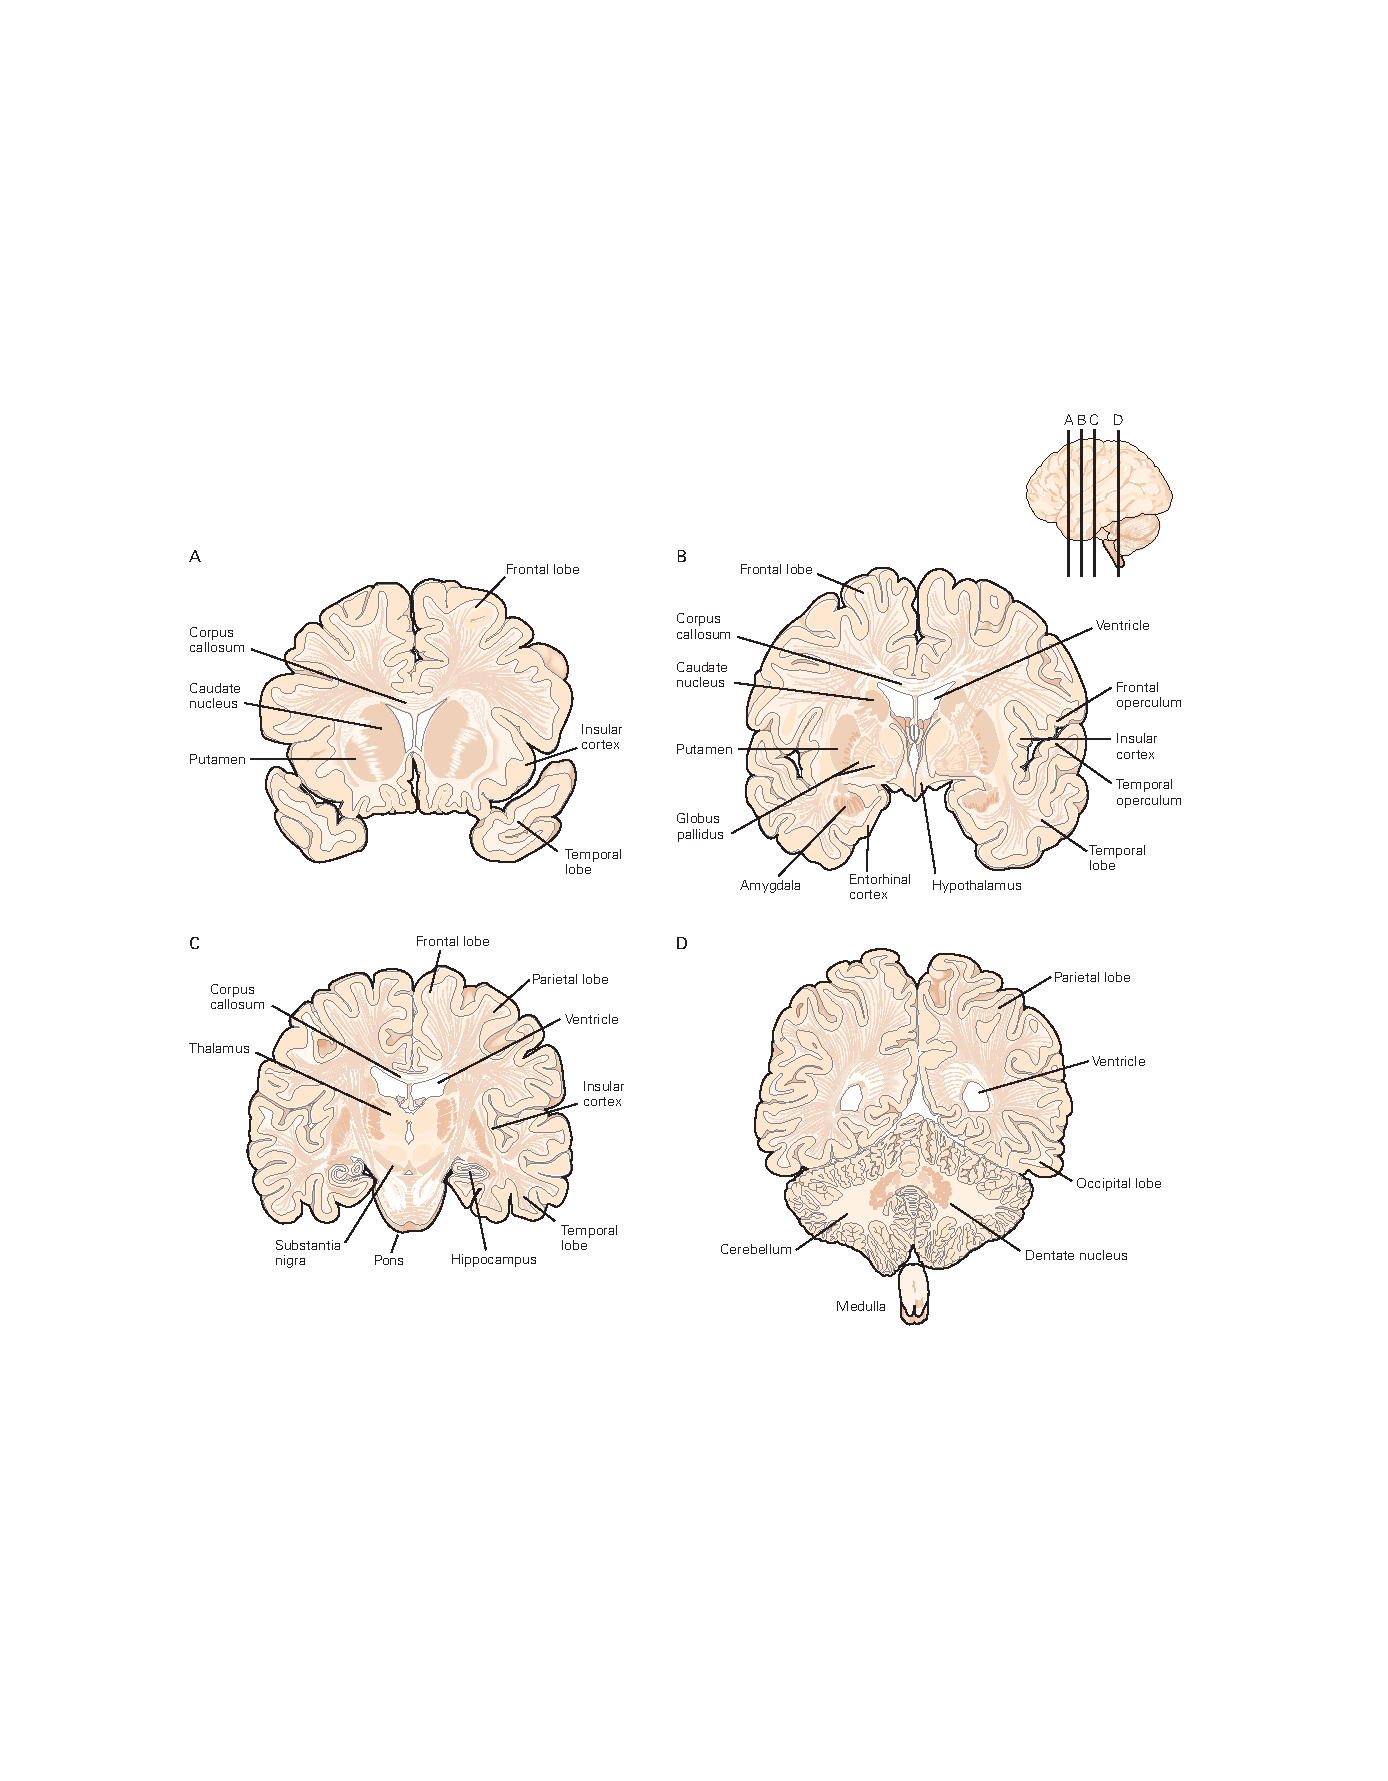
\includegraphics[width=1.0\linewidth]{chap01/fig_1_4}
	\caption{中枢神经系统的划分。
		\textbf{A.} 中枢神经系统可分为七个主要区域,从最尾部的脊髓区域,到脑干(延髓、脑桥和中脑),到间脑(包括丘脑和下丘脑),到端脑或大脑(大脑皮层、底层白质、皮层下核和基底神经节)。
		\textbf{B.} 大脑的四个主要叶以覆盖它们的颅骨部分命名。
		这张大脑的侧视图仅显示左侧大脑半球。
		中央沟将额叶和顶叶分开。
		外侧沟将额叶与颞叶分开。
		初级运动皮层占据紧靠中央沟头端的回。
		初级体感皮层占据中央沟尾部的回。
		\textbf{C.} 在右半球的内侧视图中,当半球分开时,可以看到大脑的进一步分裂。
		\textit{胼胝体}包含一大束连接两个半球的轴突。
		扣带皮层是大脑皮层的一部分,围绕着大脑皮层。
		初级视觉皮层占据距状沟。}
	\label{fig:1_3}
\end{figure}


\begin{figure}[htbp]
	\centering
	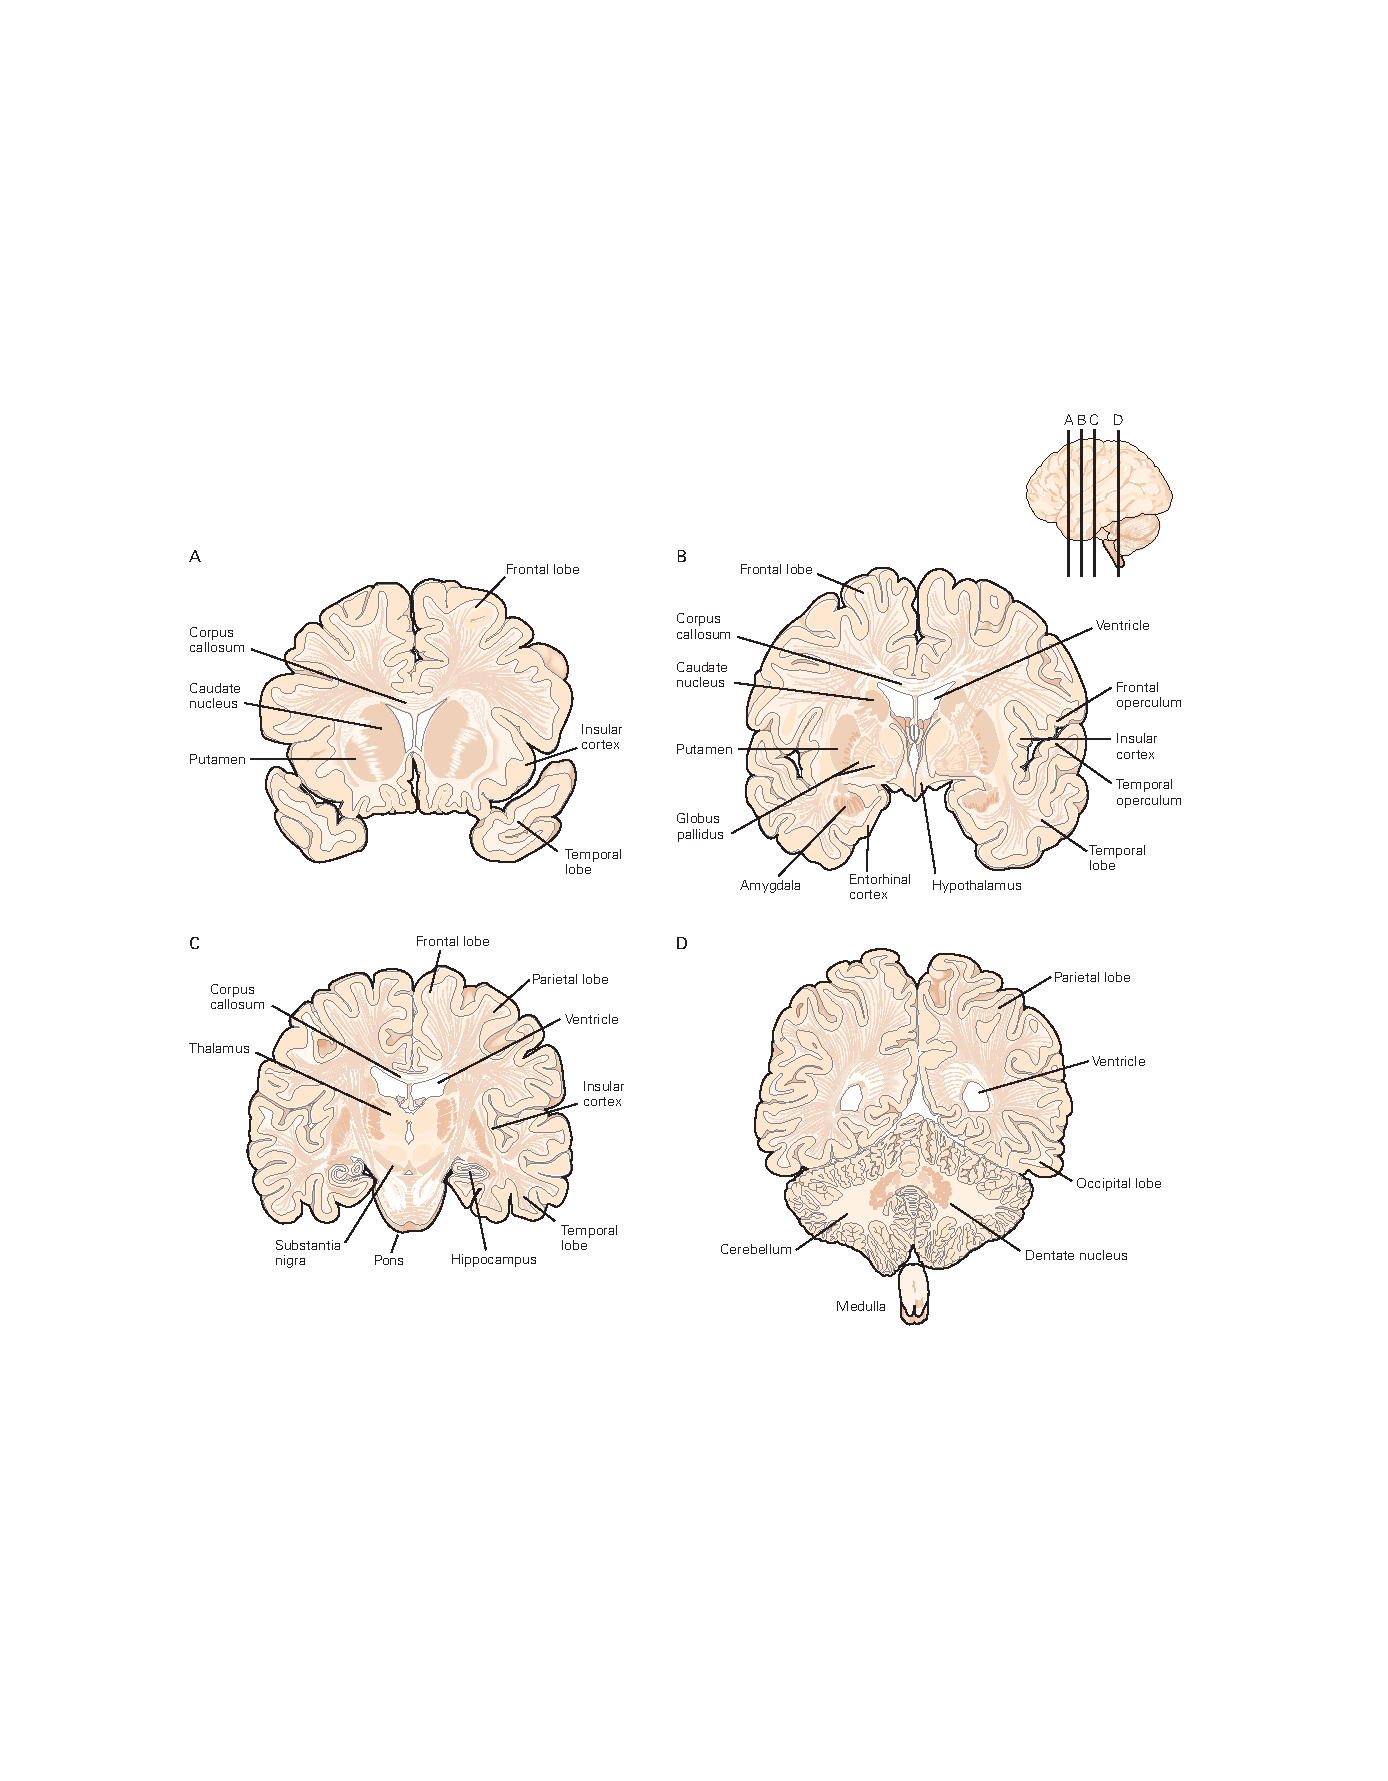
\includegraphics[width=1.0\linewidth]{chap01/fig_1_4}
	\caption{在死后组织的脑切片图中可以看到大脑半球的主要皮层下和深部皮层区域。
		四个连续的冠状切片(A–D)沿着大脑侧视图(右上角,插图)上指示的延髓-尾轴制作。
		基底神经节包括尾状核、壳核、苍白球、黑质和底丘脑核(未显示)。
		丘脑将感觉信息从外围传递到大脑皮层。
		杏仁核和海马体是埋藏在颞叶内的大脑皮层区域,对情绪反应和记忆很重要。
		脑室包含并产生脑脊液,脑脊液浸润脑沟、脑池和脊髓\cite{nieuwenhuys2007human}。}
	\label{fig:1_4}
\end{figure}


现代脑成像技术可以看到活人这些结构的活动(见第~\ref{chap:chap6}~章)。
当人们在受控条件下从事特定任务时,脑成像通常用于评估大脑离散区域的代谢活动。
这些研究提供的证据表明,特定类型的行为比其他行为更能激发大脑特定区域的活动。
大脑成像生动地表明认知操作主要依赖于大脑皮层,即覆盖两个大脑半球的皱纹灰质(图~\ref{fig:1_5})。


\begin{figure}[htbp]
	\centering
	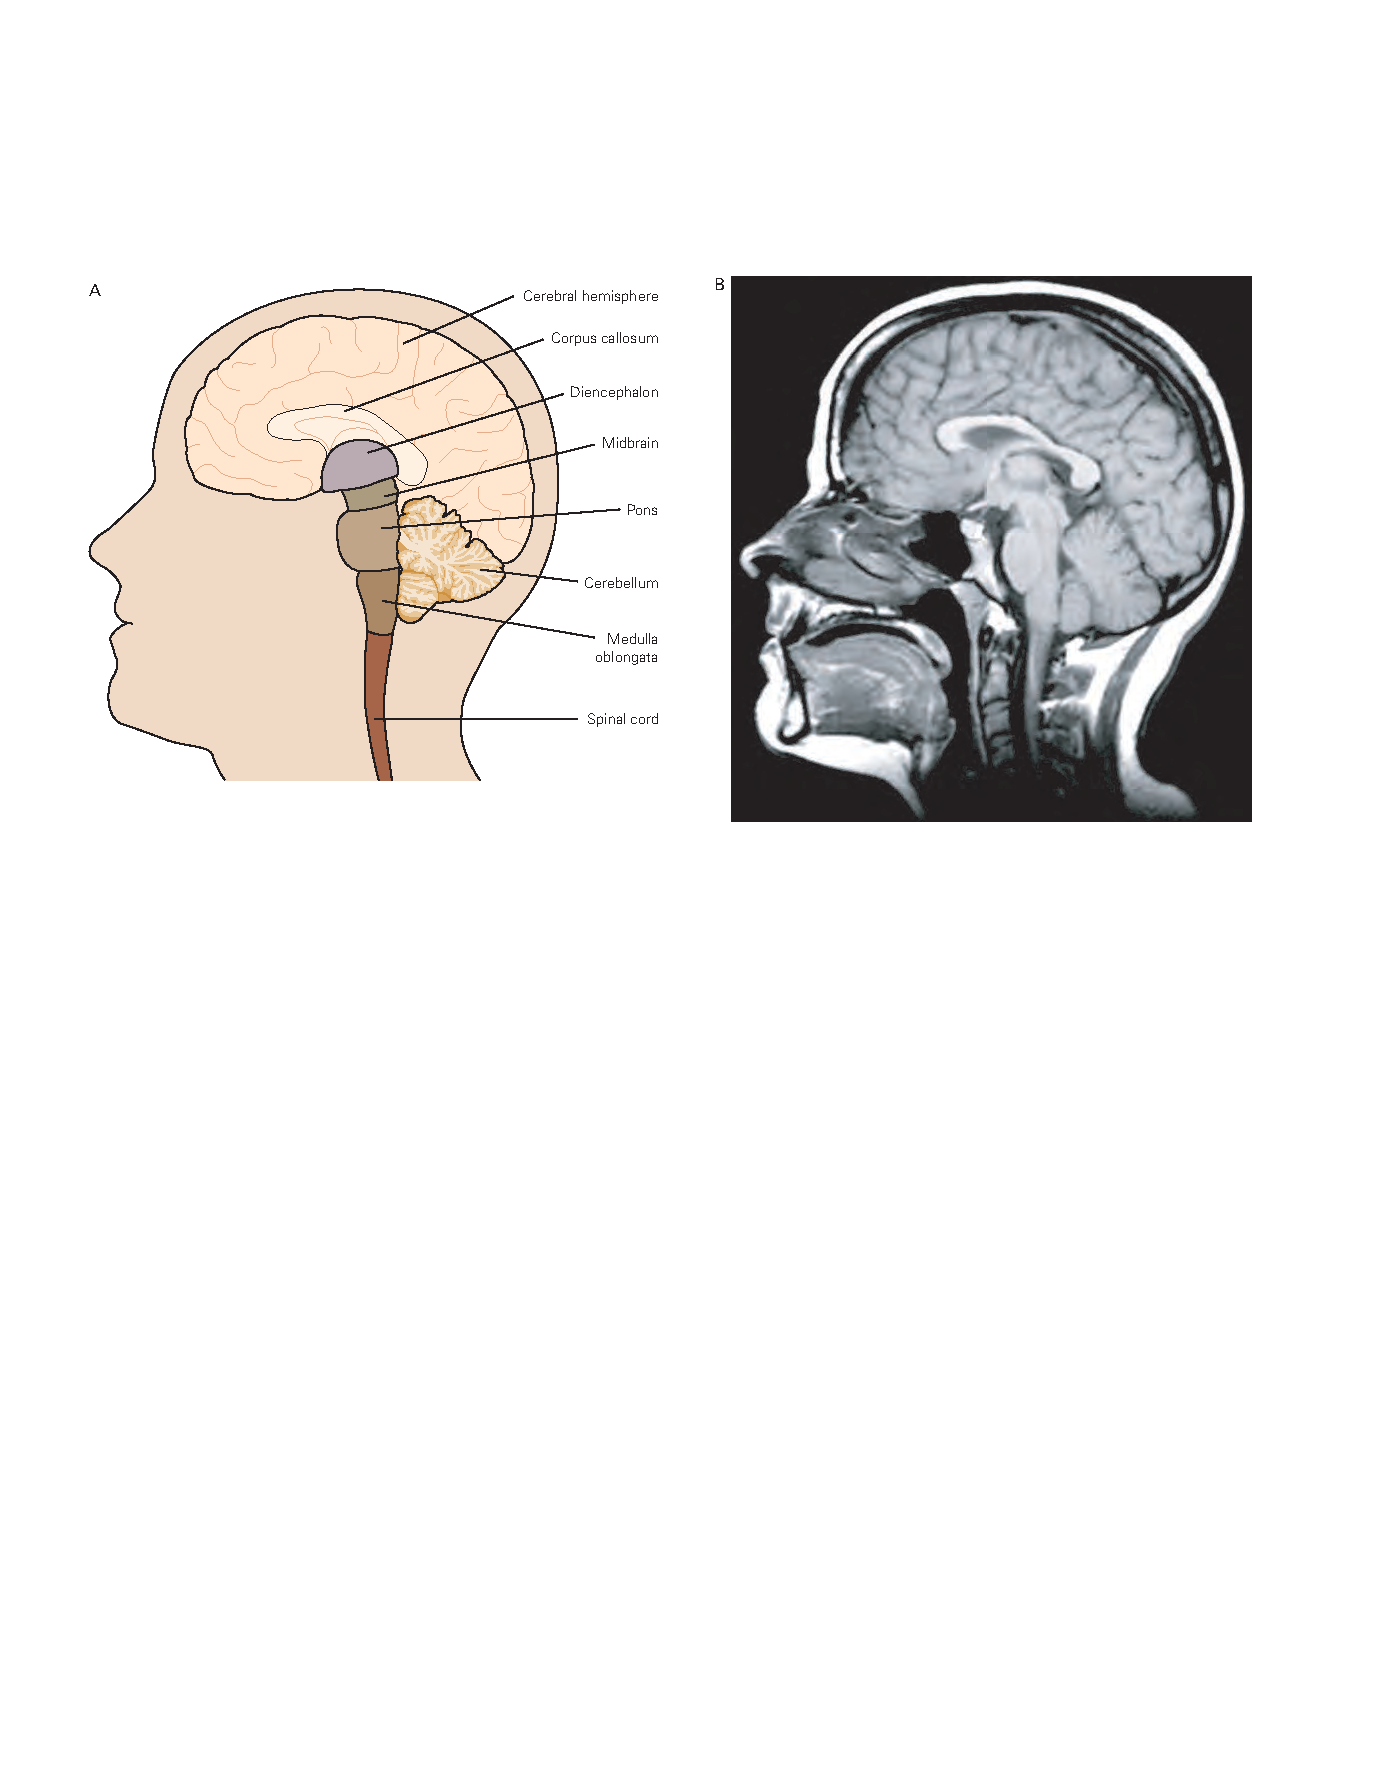
\includegraphics[width=1.0\linewidth]{chap01/fig_1_5}
	\caption{可以在活人的大脑中成像主要皮层和皮层下区域。
		\textbf{A.} 这张示意图显示了大脑的主要表面和深部区域,包括脊髓的延髓末端,以供参考。
		\textbf{B.} 在 A 部分绘制的主要大脑分区在活人脑的磁共振图像中很明显。}
	\label{fig:1_5}
\end{figure}


在每个半球中,覆盖的皮层分为四个叶,以覆盖它们的颅骨命名:额叶、顶叶、枕叶和颞叶(图~\ref{fig:1_3}B)。
每个叶都有几个特征性的深折叠,这是一种将一大片皮层包装到有限空间中的进化策略。
这些回旋的顶部称为脑回,中间的沟称为脑沟或裂隙。 
人与人之间非常相似的更突出的脑回和脑沟具有特定的名称。
例如,中央沟将中央前回(一个与运动功能有关的区域)与中央后回(一个处理感觉功能的区域)分开(图~\ref{fig:1_3}B)。
如第~\ref{chap:chap6}~章所述,无论是在死后组织中(图~\ref{fig:1_4}),还是实际上使用磁共振成像(图~\ref{fig:1_5}),几个突出的脑回仅在两个半球之间的内侧表面可见(图~\ref{fig:1_3}C),其他脑回位于脑裂和脑沟深处,因此只有在大脑被切片时才可见。


每个叶都有专门的功能。
额叶主要与短期记忆、计划未来行动和控制运动有关;
顶叶介导躯体感觉,形成身体形象并将其与个人以外的空间联系起来;
枕叶与视觉有关;
颞叶处理听觉、物体和面孔的识别,以及通过其深层结构、海马体和杏仁核处理学习、记忆和情感。


两个重要特征表征了大脑皮层的组织。
首先,每个半球主要关注身体对侧(对侧)的感觉和运动过程。
因此,从身体左侧到达脊髓的感觉信息在到达大脑皮层的途中穿过神经系统的右侧。
同样,右半球的运动区控制着身体左半边的运动。
第二个特征是两个半球虽然外观相似,但在结构或功能上并不完全对称。



\section{认知能力本地化的第一个有力证据来自语言障碍研究}

大脑皮层中第一个被确定为对认知很重要的区域是与语言有关的区域。
这些发现来自对失语症的研究,失语症是一种语言障碍,最常发生在大脑组织的某些区域因中风、供应大脑半球一部分的血管闭塞或破裂而受损时。
失语症研究中的许多重要发现
在 19 世纪下半叶,接二连三地出现许多重要的失语症研究。
总而言之,这些进展构成了人类行为神经科学研究中最激动人心和最重要的章节之一。


法国神经学家布罗卡是第一个确定与语言有关的大脑特定区域的人。
\textit{布洛卡}受到\textit{加尔}绘制大脑高层功能图的影响,但他没有将行为与头骨上的肿块相关联,而是将失语症的临床证据与死后发现的脑损伤相关联。
1861 年,他写道:“我曾认为,如果有一门颅相学,那将是(大脑皮层中)脑回的颅相学,而不是(头上的)肿块的颅相学。” 
基于这种洞察力,布罗卡创立了神经心理学,这是一门心理过程的经验科学,他将其与加尔的颅相学区分开来。


1861 年,布罗卡描述了一位名叫勒博涅的病人,他由于中风而无法说话,尽管他能很好地理解语言。
该患者没有影响其说话能力的舌头、嘴巴或声带运动缺陷。
事实上,他可以毫无困难地说出孤立的单词、吹口哨和唱出一段旋律。
但他不能按语法说话或造出完整的句子,也不能用书面表达思想。
对这名患者的大脑进行的尸检显示,左额叶后下方区域有一个病变,现在称为布罗卡区(图~\ref{fig:1_6})。
\textit{布洛卡}研究了 8 名相似的患者,均在该区域有病变,并且每个病例的病变都位于左侧大脑半球。
这一发现促使\textit{布洛卡}在 1864 年宣布:“我们用左半球说话!” 。


\begin{figure}[htbp]
	\centering
	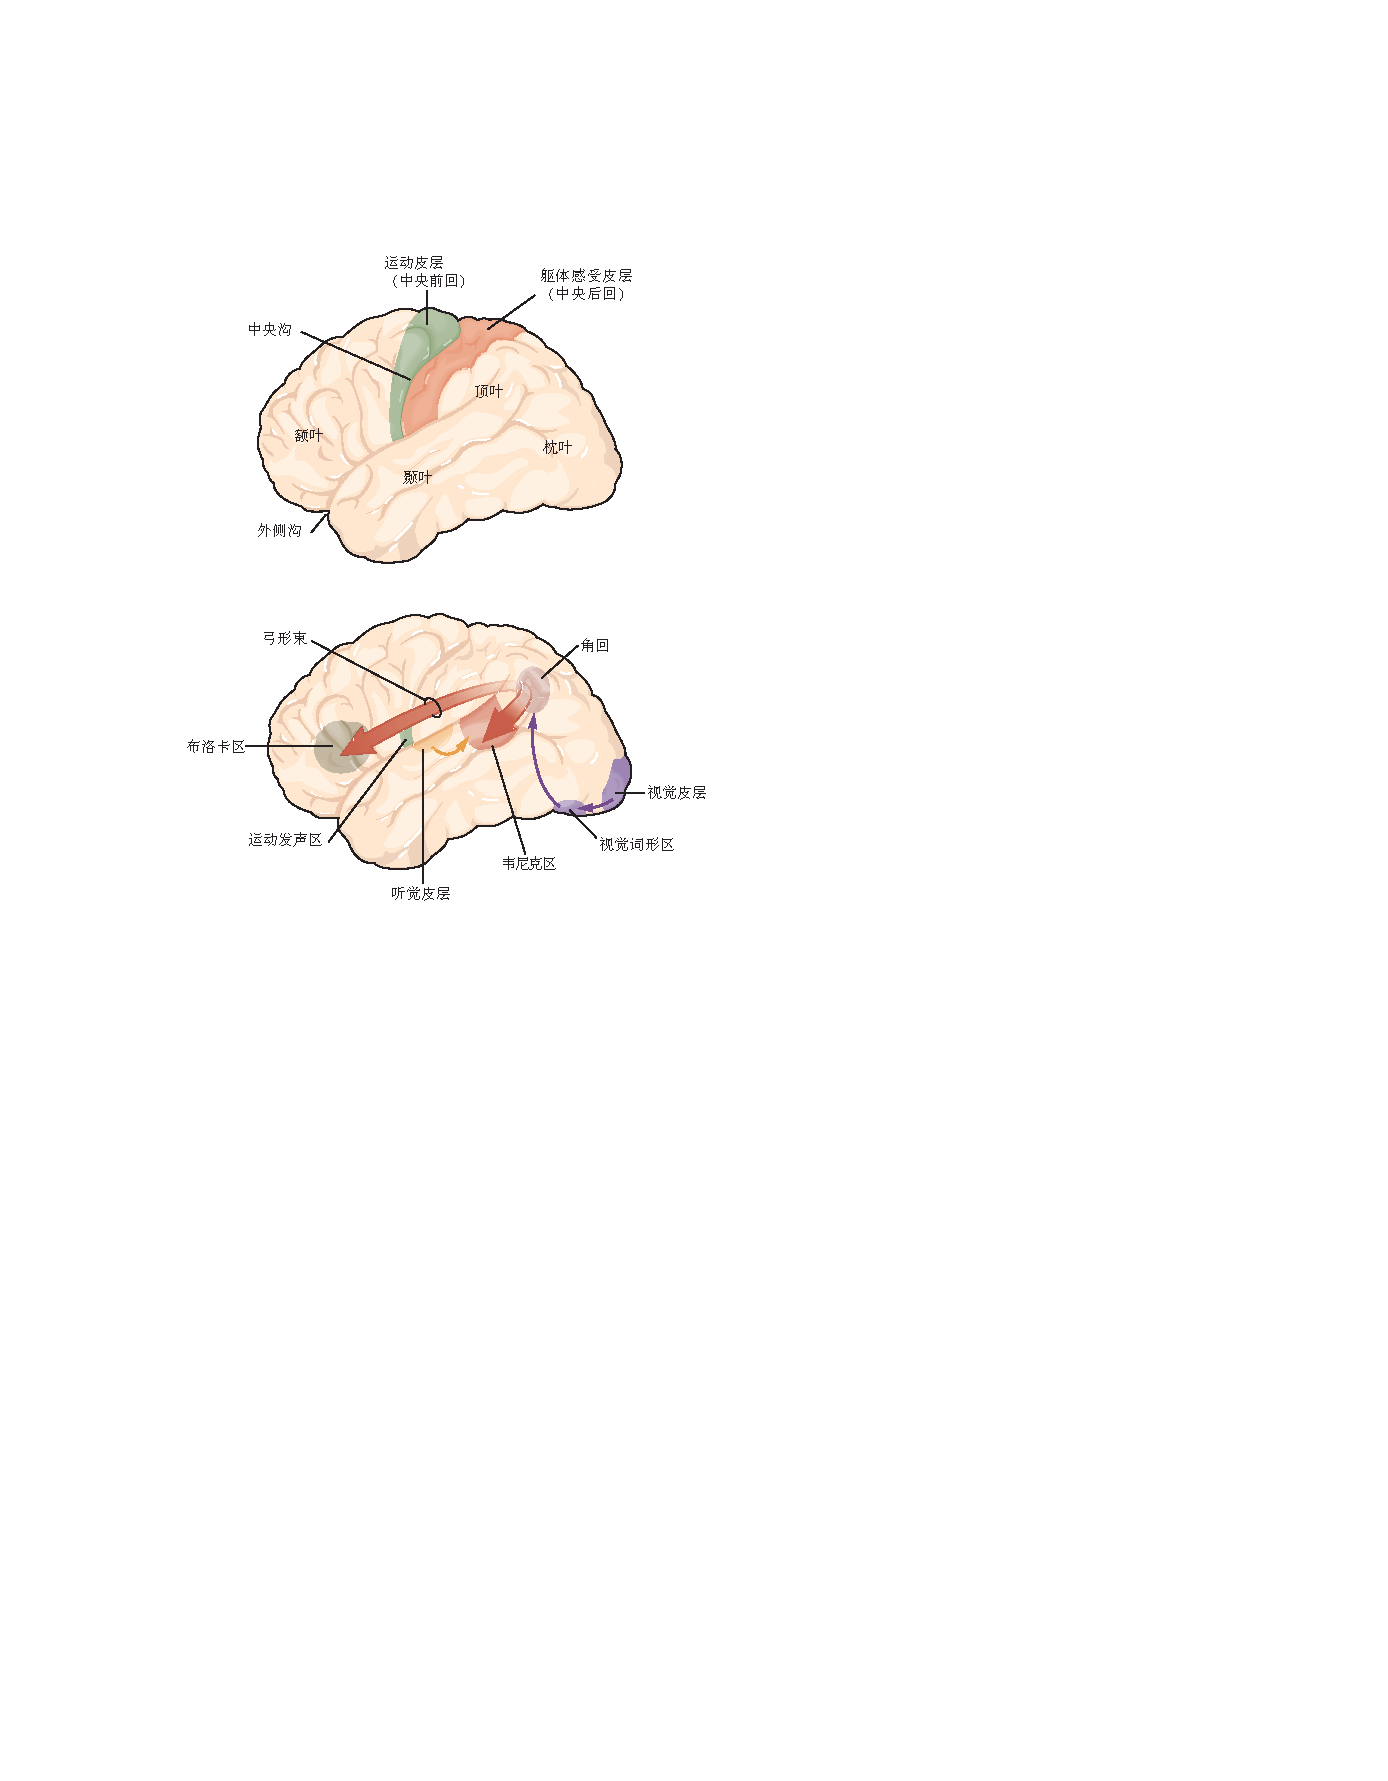
\includegraphics[width=0.7\linewidth]{chap01/fig_1_6}
	\caption{语言处理涉及左脑半球的几个区域。
		布洛卡区控制言语的产生。
		它位于控制形成单词的嘴巴和舌头运动的运动区附近。
		韦尼克区处理语言的听觉输入,对理解言语很重要。
		它位于初级听觉皮层和角回附近。
		法国神经学家\textit{朱尔斯$\cdot$代热林}在 1890 年代提出,角回中的多模态感觉区域整合了来自视觉和听觉的信息来表示单词,但最近的研究表明更多的腹侧枕颞皮层区域用于处理视觉单词。
		\textit{韦尼克}区通过双向通路与\textit{布洛卡}区相通,其中一部分由弓状束组成\cite{geschwind1979specializations}。}
	\label{fig:1_6}
\end{figure}


\textit{布洛卡}的工作激发了人们对与其他特定行为相关皮层部位的搜索,而且搜索很快就得到了回报。
1870 年,\textit{古斯塔夫$\cdot$弗里奇}和\textit{爱德华$\cdot$希茨格}表明,可以通过电刺激中央前回的离散区域来产生狗的特征性肢体运动,例如伸出爪子,这激起了科学界的热潮。
这些区域总是位于对侧运动皮层。
因此,最常用于书写和熟练动作的右手是由左半球控制的,而左半球也控制着说话。
因此,对大多数人来说,左半球被认为是主导的。


下一步是由\textit{韦尼克}于 1876 年采取的,他在 26 岁时发表了一篇现在已成为经典的论文,“失语症的综合症状:解剖学基础上的心理学研究”。
在其中,他描述了另一种类型的失语症,这是一种理解障碍而不是言语障碍:一种与表达障碍相反的接受障碍。
布罗卡的病人可以理解语言但不会说话,而韦尼克的病人可以造词但不能理解语言,只能说出毫无意义但合乎语法的句子。
而且,这种新型失语症的发生部位与布罗卡所描述的不同。
病变发生在大脑皮层后部,即颞叶与顶叶交汇处(图~\ref{fig:1_6})。


基于这一发现以及\textit{布洛卡}、\textit{弗里奇}和\textit{希茨格}的工作,\textit{韦尼克}制定了一种语言神经模型,试图调和和扩展当时大脑功能的主流理论。
颅相学家和细胞联结主义者认为,大脑皮层是功能特定区域的马赛克,而整体聚合场学派则声称,每一种心理功能都涉及整个大脑皮层。
韦尼克提出,只有最基本的心理功能,即与简单的知觉和运动活动有关的功能,才完全由皮层离散局部区域的神经元调节。
他认为,更复杂的认知功能是由几个功能部位之间的相互联系产生的。
通过将局部功能原理整合到联结主义框架中,韦尼克强调了单一行为的不同组成部分可能在大脑的多个区域中得到处理的观点。
因此,他是第一个提出分布式处理思想的人,分布式处理现在是神经科学的核心原则。


\textit{韦尼克}假设语言涉及独立的运动和感觉程序,每个程序都由不同的皮层区域控制。
他提出,控制言语嘴部运动的运动程序位于\textit{布罗卡区},恰好位于控制嘴、舌、上颚和声带的运动区的前面(图~\ref{fig:1_6})。
接下来,他将控制单词感知的感觉程序分配到他发现的颞叶区域,现在称为韦尼克区。
该区域被听觉皮层和现在统称为联合皮层的区域包围,这些区域整合了听觉、视觉和躯体感觉。
根据\textit{韦尼克}的模型,这两个语言中心之间的交流是通过一大束被称为弓状束的轴突来调节的。


因此,韦尼克制定了第一个连贯的语言神经模型,该模型在第~\ref{chap:chap55}~章中进行了重要的修改和阐述,至今仍然有用。
根据这个模型,口语或书面词的神经处理开始于专门负责听觉的皮层的单独感觉区域 或视觉信息。
然后,通过中间关联区域提取适合口头或书面文字识别的特征,将此信息传送到韦尼克区,在那里它被识别为语言并与意义相关联。


韦尼克模型的强大之处不仅在于它的完整性,还在于它的预测效用。
该模型正确预测了第三种类型的失语症,一种由断开连接引起的失语症。
在这种类型中,语言的感受区和表达区完好无损,但连接它们的神经纤维(弓状束)被破坏。
这种传导性失语症,正如现在所称,其特征是频繁的、基于声音的言语错误(音素性错语)、重复困难和言语工作记忆的严重限制。
传导性失语症患者能理解他们听到和读到的单词,并且在说话时没有运动障碍。
然而,他们无法连贯地说话; 他们省略部分单词或替换不正确的声音,并且在逐字重复他们听到、读到或从记忆中回忆起的多音节单词、短语或句子时遇到很大困难。
尽管他们痛苦地意识到自己的错误,但他们连续不断的自我纠正尝试往往都没有成功。


在解剖学家布罗德曼的领导下,部分受到韦尼克的启发,20 世纪初在德国出现了一个新的皮层定位学派,该学派根据细胞的形状及其分层的变化来区分皮层的功能区域 安排。
使用这种细胞构造方法,布罗德曼区分了人类大脑皮层中 52 个解剖学和功能上不同的区域(图~\ref{fig:1_7})。


\begin{figure}[htbp]
	\centering
	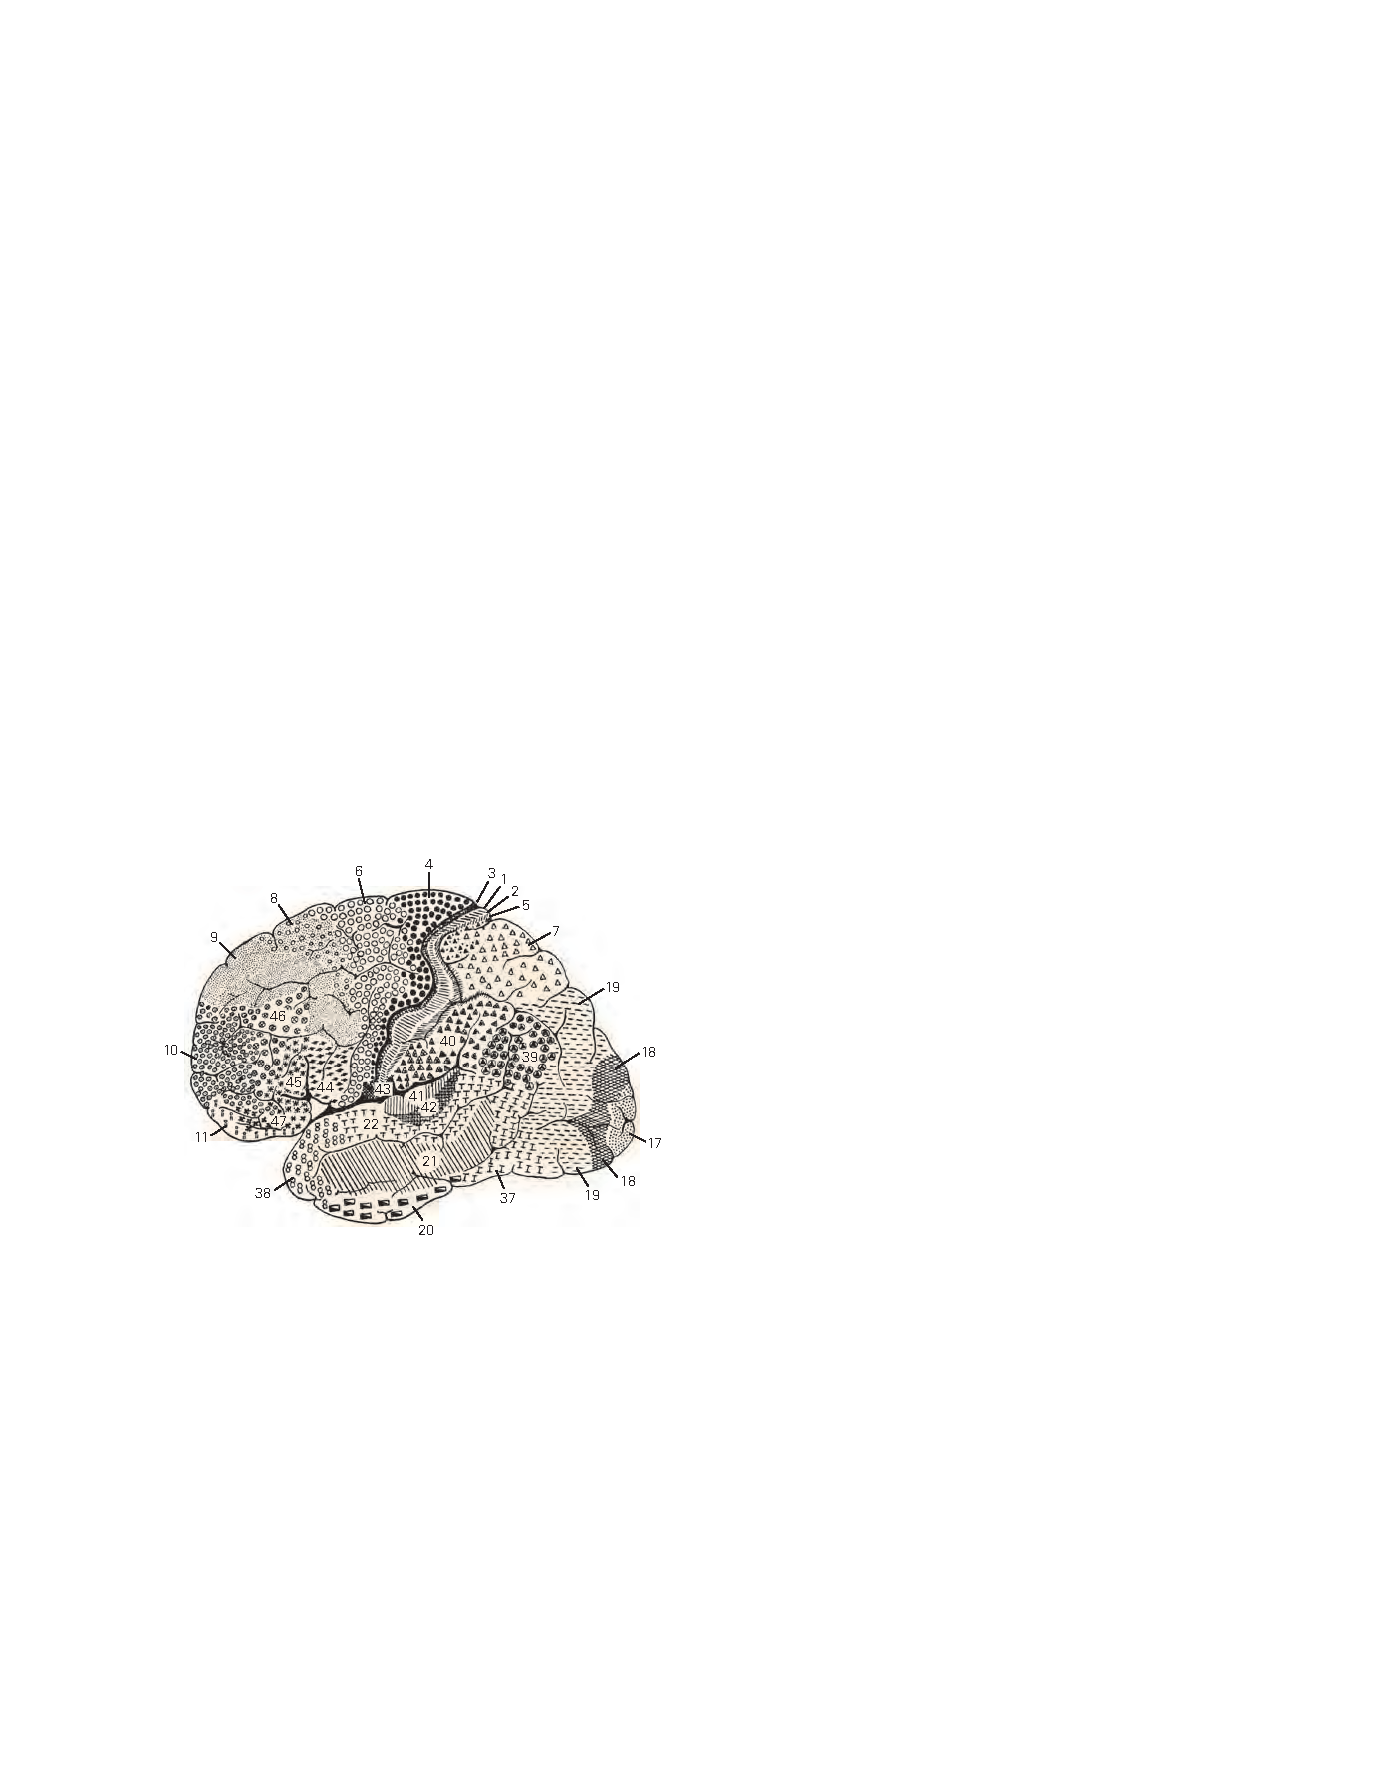
\includegraphics[width=0.65\linewidth]{chap01/fig_1_7}
	\caption{20 世纪初,人类大脑皮层被分为 52 个独立的功能区。
		显示的区域是由解剖学家布罗德曼根据独特的神经细胞结构和细胞层的特征排列确定的。
		该方案至今仍在广泛使用,并不断更新。
		布罗德曼定义的几个区域被发现可以控制特定的大脑功能。
		例如,区域 4 是运动皮层,负责随意运动。
		区域 1、2 和 3 构成初级体感皮层,主要从皮肤和关节接收感觉信息。
		第 17 区是初级视觉皮层,它接收来自眼睛的感觉信号并将它们传递到其他区域以进行进一步处理。
		区域 41 和 42 构成初级听觉皮层。
		该图仅显示了皮层外表面的可见区域。}
	\label{fig:1_7}
\end{figure}


尽管大脑皮层功能离散区域的生物学证据令人信服,但到 20 世纪初,大脑的整体观点一直主导着实验思维和临床实践,直到 1950 年。
这种令人惊讶的事态在很大程度上要归功于几位著名的神经科学家,他们 主张整体观的有英国神经学家亨利海德、俄国行为生理学家伊万巴甫洛夫和美国心理学家卡尔\textit{拉什利}。


最有影响力的是\textit{拉什利},他对用细胞构造方法来绘制皮层功能图深表怀疑。
“‘理想’的建筑地图几乎一文不值,”\textit{拉什利}写道。
“区域划分在很大程度上在解剖学上毫无意义,并且对皮层的假定功能划分具有误导性。” 
他对各种脑损伤对老鼠学习走迷宫能力的影响的研究进一步强化了他的怀疑态度。
从这些研究中,\textit{拉什利}得出结论,学习缺陷的严重程度取决于损伤的大小,而不是其精确位置。
失望的\textit{拉什利}(以及他之后的许多其他心理学家)得出结论,学习和其他高层心理功能在大脑中没有特殊的位置,因此不能归因于特定的神经元集合。


根据他的观察,\textit{拉什利}通过进一步最小化单个神经元、特定神经元连接,甚至特定大脑区域在特定行为中产生的作用,重新制定了聚合场观点。
根据\textit{拉什利}的质量作用理论,对记忆等功能至关重要的是大脑的整体质量,而不是其局部成分。


\textit{拉什利}的老鼠实验现在被重新诠释。
各种研究表明,\textit{拉什利}使用的迷宫学习不适合寻找局部皮层功能,因为它涉及太多的运动和感觉能力。
被剥夺了一种感觉能力,比如视觉,老鼠仍然可以学会使用触觉或嗅觉走迷宫。
此外,正如我们将在本书后面看到的那样,许多心理功能是由不止一个区域或神经元通路调节的。
因此,一个给定的功能可能不会被单个损伤消除。
在考虑大脑的认知功能时,这一点尤为重要。
例如,空间知识得到许多顶叶关联区域的支持,这些关联区域将视觉与注视的潜在移动、头部的转动、手的伸展等联系起来。
原则上,这些关联区域中的任何一个都可以补偿另一个关联区域的损伤。
对顶叶的严重损伤会导致明显的空间知识缺陷(空间失认症)(第~\ref{chap:chap59}~章)。
这样的观察似乎支持群众行动理论,但我们现在认识到它与包含功能冗余概念的功能定位相容。


很快,功能定位的证据变得势不可挡。
从 1930 年代后期开始,英国的\textit{埃德加$\cdot$阿德里安}和美国的\textit{韦德$\cdot$马歇尔}和\textit{菲利普$\cdot$巴德}发现,触摸猫身体的不同部位会引起大脑皮层不同区域的电活动。
通过系统地探测体表,他们在\textit{布罗德曼}描述的大脑皮层特定区域建立了体表的精确图谱。
这一结果表明,可以根据解剖学标准(例如细胞类型和细胞分层、细胞连接,以及最重要的行为功能)明确定义功能不同的皮层区域。
正如我们将在后面的章节中看到的那样,功能特化是大脑皮层的一个关键组织原则,甚至延伸到皮层区域内的单个细胞列。
事实上,大脑被划分为比布罗德曼设想的更多的功能区域。


更精细的方法使我们有可能更多地了解与语言有关的不同大脑区域的功能。
在 20 世纪 50 年代后期,\textit{怀尔德$\cdot$潘菲尔德}和后来的\textit{乔治$\cdot$奥杰曼}重新研究了对产生语言至关重要的皮层区域。
在癫痫脑部手术期间进行局部麻醉时,清醒的患者被要求命名物体(或以其他方式使用语言),同时用小电极刺激暴露皮层的不同区域。
如果大脑皮层的某个区域对语言至关重要,则电刺激的应用会阻止患者命名物体的能力。
通过这种方式,\textit{潘菲尔德}和\textit{奥杰曼}能够确认 布洛卡和韦尼克描述的大脑皮层的语言区域。
正如我们将在第~\ref{chap:chap55}~章中了解到的那样,语言神经网络比布洛卡和韦尼克所描述的神经网络广泛和复杂得多。


最初,几乎所有关于语言解剖结构的知识都来自对脑部病变患者的研究。
今天,\textit{功能性磁共振成像}和其他非侵入性方法可以对从事阅读、说话和思考的健康人进行分析(第~\ref{chap:chap6}~章)。
\textit{功能性磁共振成像}不仅证实了阅读和说话会激活不同的大脑区域,而且还揭示了在没有感觉输入的情况下仅仅思考一个词的含义会激活左额叶皮层中一个仍然不同的区域。
事实上,即使在传统语言领域内,各个子区域也会在不同程度上被吸收,这取决于我们思考单词、表达单词以及从其他单词的排列(即句法)中解析它们的含义的方式。
新的成像工具承诺不仅会告诉我们涉及哪些领域,还会揭示它们相互联系的功能逻辑。


现代方法论带来的巨大惊喜之一是,大脑皮层的如此多区域在语言理解和产生过程中都被激活了。
这些包括左半球的传统语言区域,由\textit{布洛卡}、\textit{韦尼克}和\textit{代热林}确定; 它们在右半球的同系物;
和新确定的区域。
功能成像倾向于阐明不同募集的区域,而来自中风、肿瘤或损伤的损伤区分对一种或多种功能至关重要的大脑区域。
因此,曾经被认为专门负责语言生成的布罗卡区似乎也参与了包括理解在内的各种语言任务(图~\ref{fig:1_6})。
在某些情况下,功能成像需要对病变研究确定的关键区域进行改进或修正。
例如,除了顶叶皮层的角回之外,阅读现在被认为可以募集腹侧枕颞皮层的专门区域(如图~\ref{fig:1_6} 所示)。


因此,大脑中语言的处理不仅体现了局部功能原则,而且体现了这一原则的更复杂的阐述,即许多具有专门功能的不同神经结构属于系统。
也许这是关于本地化和分布式过程争论的自然调和,即少数不同的区域,每个区域都具有一小组功能,并通过它们的相互作用对感知、行动和观念的现象学做出贡献。
大脑分工的任务可能与我们的直觉告诉我们的不同。
谁会猜到对一个物体的运动和颜色的神经分析会发生在不同的通路中,而不是一个单一的通路来调解对物体的统一感知?
同样,我们可能期望语言的神经组织可能不完全符合通用语法理论的公理,但支持语言理论描述的非常无缝的功能。


对脑损伤患者的研究继续提供重要的洞察力,以了解大脑是如何组织语言的。
最令人印象深刻的结果之一来自对聋人的研究,他们在遭受脑损伤后失去了使用手语(例如,\textit{英国手语}或\textit{美国手语})进行交流的能力。
手语使用手部动作而不是发声,并且通过视觉而不是声音来感知,但具有与口语相同的结构复杂性。
与口语处理一样,手语处理位于左半球。 左半球的损伤会对手语产生非常特殊的影响,就像口语一样,会影响手语理解(韦尼克区受损后)、语法或流畅性(布罗卡区受损后)。
这些临床观察得到功能性神经影像学的支持。
毫不奇怪,手语和口语的产生和理解并不涉及相同的大脑区域,但重叠确实很显著(图~\ref{fig:1_8})。
甚至有证据表明,处理符号的组成部分(例如,使用的手形)涉及的一些相同大脑区域在对语音进行押韵判断时涉及。


\begin{figure}[htbp]
	\centering
	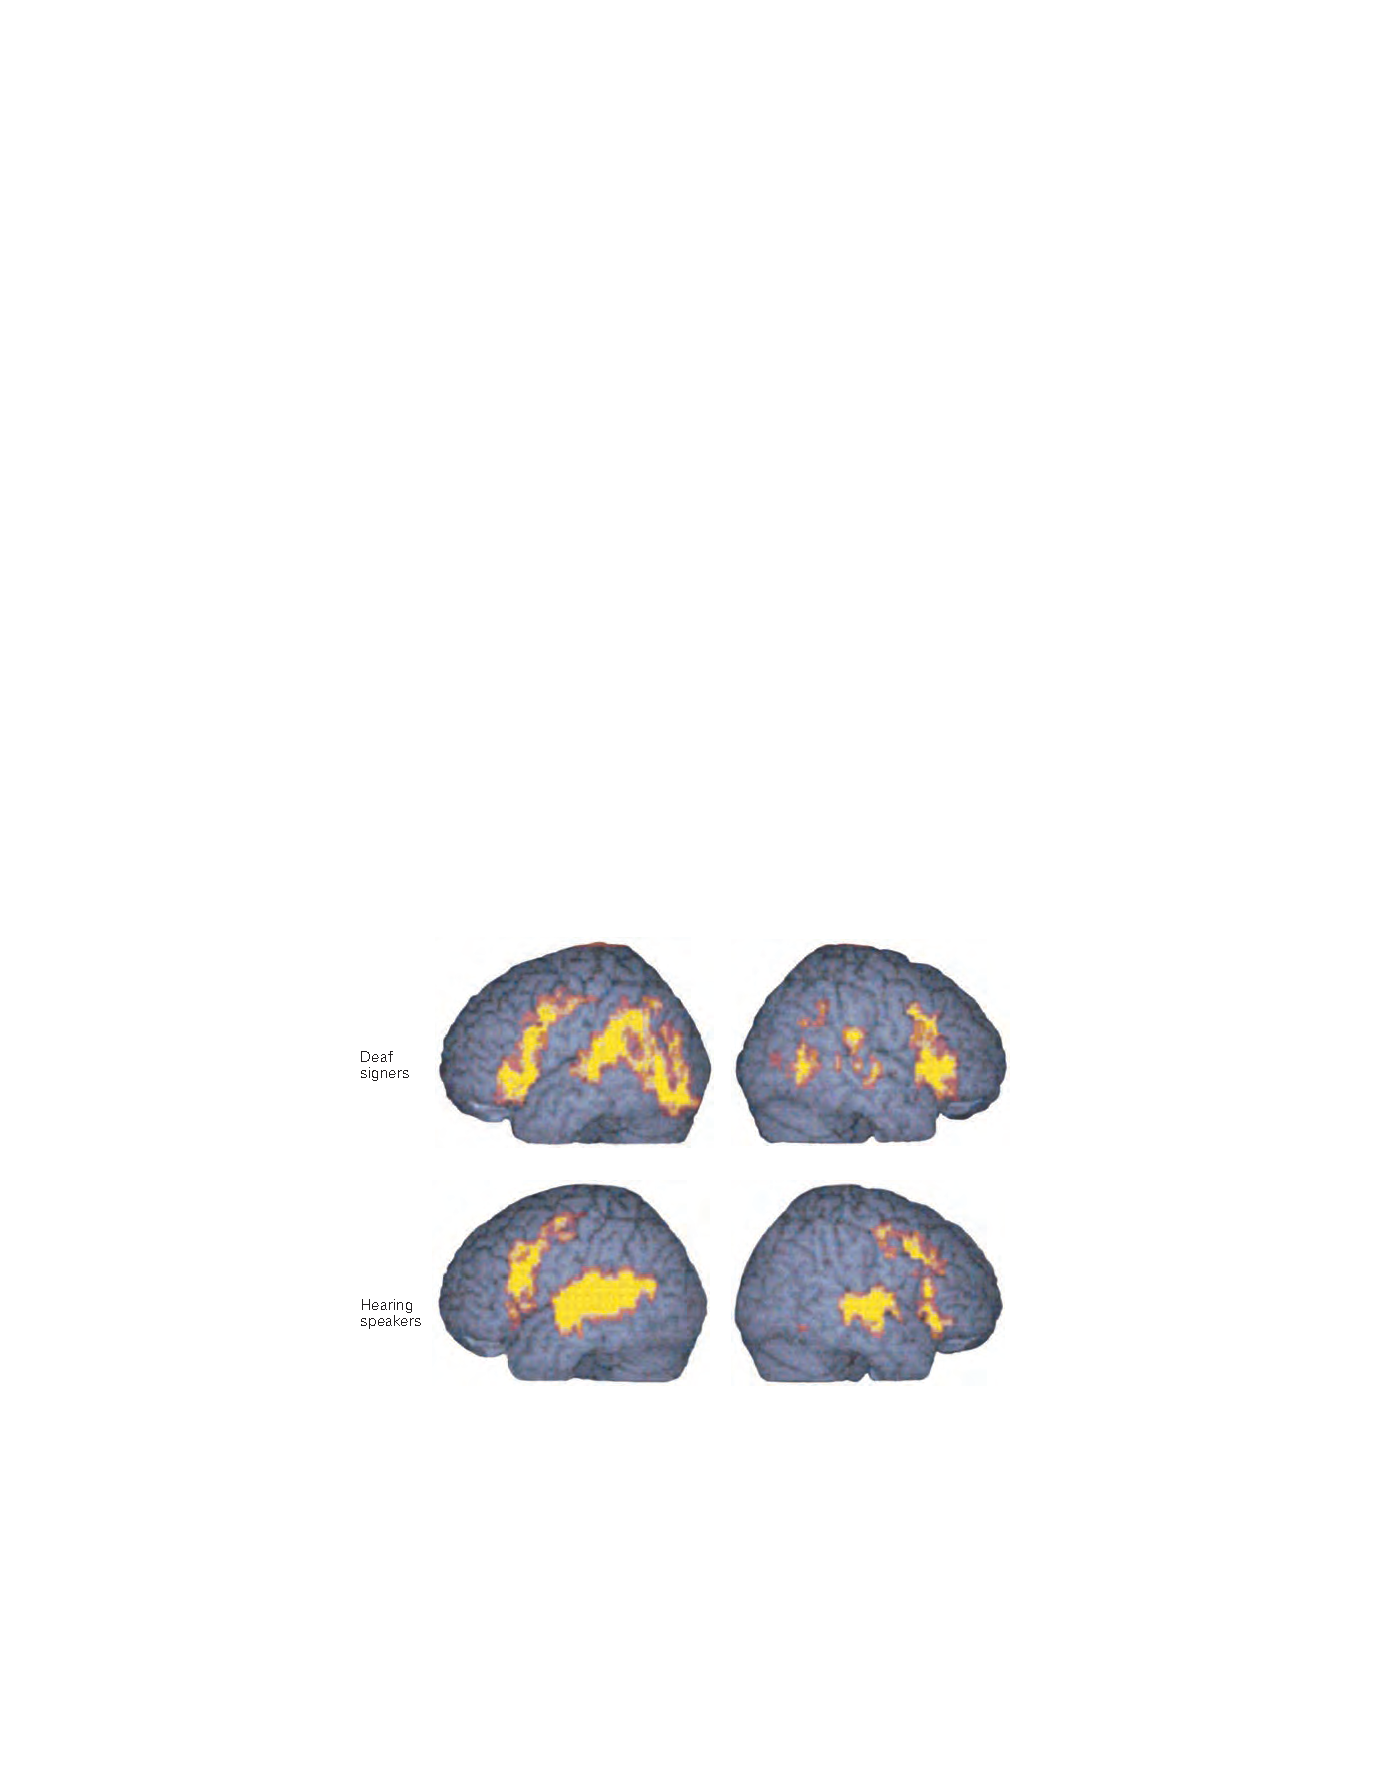
\includegraphics[width=0.82\linewidth]{chap01/fig_1_8}
	\caption{手语聋人和听力正常的人共享共同的语言处理区域。
		大脑皮层中涉及口语或手语识别的区域,通过\textit{功能性磁共振成像}识别。
		黄色高亮显示左右大脑半球(分别为左列和右列)在理解语言时比在执行感知任务时更活跃的区域。
		对于失聪手语者(顶行),突出显示的区域在理解英国手语期间比在检测叠加在同一静止手语者身上的视觉刺激期间更加活跃。
		对于有听力的说话者(下排),在理解视听语音期间突出显示的区域比在观看静止(无声)说话者时检测音调期间更活跃\cite{macsweeney2002neural}。}
	\label{fig:1_8}
\end{figure}


这些观察说明了三点。
首先,语言处理主要发生在左半球,与处理语言中使用的感觉和运动方式的通路无关。
其次,听觉输入对于左半球语言能力的出现和运作不是必需的。
第三,口语只是左半球调节的一系列语言技能之一。


对其他行为的调查为大脑具有不同认知系统的观点提供了额外的支持。
这些研究表明,复杂的信息处理需要许多相互关联的皮层和皮层下区域,每个区域都涉及处理感觉刺激或运动的特定方面,而不是其他方面。
例如,对物体位置、大小和形状的知觉意识依赖于许多顶叶联合区域的活动,这些区域将视觉与潜在的动作联系起来,例如移动眼睛、调整头部方向、伸手和调整手的形状以进行抓握。
顶叶区域不会启动这些动作,但会将感觉信息评估为与这些潜力相关的证据。
它们从背侧视觉流(有时称为\textit{空间通路},但更恰当地称为 how 通路)接收信息,以构建关于物体位置和其他空间特性的知晓状态。
腹侧视觉流,或什么通路,也与可能的行动有关,但这些与社交和觅食有关。
这些联想建立了对物体、面孔、食物和潜在伴侣的可取性的认知。
从这个意义上说,\textit{内容通路}也可能是 how 通路。



\section{心理过程是大脑中基本处理单元之间相互作用的产物}

大脑功能定位的证据在过去常常被拒绝,原因有很多,这些证据回想起来似乎如此明显和令人信服。
颅相学家在没有充分证据的情况下以夸张的形式引入了定位的概念。
他们把大脑皮层的每个区域都想象成一个独立的精神器官,专门负责人格完整而独特的方面,就像胰腺和肝脏是独立的消化器官一样。
\textit{弗卢龙}对颅相学的拒绝以及随之而来的聚集场观点的支持者(反对定位)和细胞连接主义者(支持定位)之间的争论是对一种简单化且没有足够实验证据的理论的回应。


在韦尼克发现大脑中语言的模块化组织(具有独特功能的互连节点)之后,我们现在认为所有认知能力都是分布在大脑多个区域的许多处理机制相互作用的结果。
也就是说,特定的大脑区域并不完全负责特定的智力,而是共同发挥作用的基本处理单元。
感知、运动、语言、思想和记忆都是通过这些区域内离散大脑区域(计算模块)中串行和并行处理的相互联系而成为可能的。
因此,单个区域的损伤不一定会像许多早期神经学家认为的那样导致认知功能(或能力)的完全丧失。
即使一种行为最初消失了,它也可能部分恢复,因为大脑未受损的部分重新组织了它们的联系。
此外,当\textit{局灶性损伤}对心理功能产生不利影响时,它可能会通过破坏其他主要位点的功能(精神分裂症)而间接影响。
事实上,对这种性质的观察让韦尼克的学生库尔特戈德斯坦接受了更全面的观点。


因此,认为心理功能严格由一系列神经细胞和大脑区域调节(每个神经细胞和大脑区域都直接连接到下一个)是不准确的,因为在这样的安排中,当单个连接受损时,整个过程就会中断。
一个更现实的比喻是一个过程,该过程由模块网络中的多个并行通路组成,这些通路相互作用并最终汇聚在一组共同的目标上。
网络中单个路径的故障可能会影响该路径携带的信息,而不会破坏整个系统。
网络的其余部分可能能够修改其性能以适应一条路径的故障。


大脑中的模块化处理被接受的速度很慢,因为直到最近,还很难证明哪些心理运算的组成部分是由特定大脑区域或通路传达的。
以导致可检验假设的方式定义心理操作也不容易。
然而,随着近几十年来现代认知心理学和脑科学的不断融合,我们已经开始意识到心理功能可以成功地分解为子功能。


为了说明这一点,请考虑我们如何学习、存储和回忆有关物体、人和事件的信息。
简单的反思表明,我们将每条知识存储为一个单一的表征,可以通过记忆慢跑刺激甚至仅通过想象力来回忆。
例如,你所知道的关于苹果的一切似乎都存储在一个完整的表征中,无论你看到一个特定的苹果、苹果的一部分、红苹果还是绿苹果、书面单词“苹果”,还是关于引力发现的虚构故事,都同样可以访问。
然而,我们的经验并不能忠实地指导知识是如何存储在记忆中的。


关于苹果的知识并没有存储为一个单一的连贯表征,而是被细分为不同的类别并单独存储。
大脑的一个区域存储着关于你拿苹果的方式、你对柔软度的感觉(与新鲜度有关)、颜色(与偏好或新鲜度相关)、你与他人交流苹果存在或味道的方式,以及它与计算机、物理学家、蠕虫、蛇和圣经花园的语义联系的信息。
“苹果”的概念包含了这些考虑因素中的每一个,还有更多。
一个自然的假设是,一个包含许多细节的连贯概念必须存在于大脑的一个单一位置;
然而,一个同样有效的假设是,像“苹果”这样的统一概念以各种神经结构之间的多重链接的形式存在于大脑中,每个神经结构都有一种特定的信息,通过记忆检索的动作进行协调。


心理过程模块化组织最惊人的例子是发现我们的自我意识(一个自我意识的存在),当我们说“我”时的意思总和,是通过我们两个大脑半球中独立回路的连接来实现的,每个回路都介导着自己的意识。
\textit{罗杰$\cdot$斯佩里}、\textit{迈克尔$\cdot$加扎尼加}和 \textit{约瑟夫$\cdot$伯根}在研究患者的过程中做出了一个非凡的发现,即意识也不是一个单一的过程,这些患者的胼胝体(连接两个大脑半球的主要区域)被切断作为治疗癫痫。
他们发现每个半球都有一种独立于另一半球运作的意识。


因此,当一名患者左手拿着一本最喜欢的书阅读时,控制左手但在语言理解中只起次要作用的右半球发现,它从简单地看书获得的原始视觉信息是无聊的。
右半球命令左手放下书。
另一个病人会用左手穿上衣服,同时用另一只手脱下衣服。 每个半球都有自己的想法!
此外,优势半球有时会评论非优势半球的表现,经常表现出一种错误的自信感,因为它不知道解决方案是专门提供给非优势半球的。


这些发现将曾经属于哲学和精神分析领域的意识研究带入了神经科学的范畴。
正如我们将在后面的章节中看到的,本章中描述的许多问题在意识的神经理论中再次出现。
没有人质疑很多信息处理(也许是最大的份额)没有达到有意识的认识这一想法。
当感官信息、行动计划或想法确实成为意识时,神经科学试图解释调节这种转变的机制。
虽然目前还没有令人满意的解释,但一些脑科学家将这一过程比作注意力焦点的转移,由不同的神经元群介导,而另一些人则认为,意识需要在广泛分离的神经元区域之间的功能相互作用中发生质的变化。


我们花了这么长时间才弄清楚大脑的哪些区域介导了哪些心理活动,主要原因是我们正在处理生物学最深奥的谜题:解释意识和自我意识的神经机制。
目前还没有令人满意的理论来解释为什么只有一些到达我们眼睛的信息会导致对物品、人或场景的主观意识状态。 
我们知道,我们有意识地意识到我们思想思考的一小部分,而那些确实刺穿意识的想法必须来自大脑无意识地执行的步骤。
正如我们在第~\ref{chap:chap56}~章中提出的那样,一些意识之谜的答案可能比想象的更接近。


同时,我们目前理解上的差距也对神经科学提出了实际的认识论挑战。
在我们对知觉、行为和认知的描述中,我们不得不依赖我们对世界、身体和观念的有意识体验。
然而,在这样做时,我们冒着错误描述许多不穿透意识的心理过程的风险。
例如,我们倾向于用与感官信息的主观体验相一致的术语来描述知觉问题,而即使是复杂但无意识的知觉内容知识也可能与行为效用(可供性)有更大的相似性,实际上是对以下问题的回答 这是否是我可能会选择吃、坐在上面或进一步参与的东西。
同样,大脑执行推理、制定战略和决策等认知过程的方式可能与我们从有意识的深思熟虑中推断出的步骤大致相似。


这些警示说明有一个明显的推论。
许多认知功能在没有意识的情况下发生的洞察力提出了这样一种可能性,即在研究更基本的行为时揭示的神经科学原理可以提供对更复杂的认知过程的洞察力。
受过训练以执行复杂任务的动物大脑的神经记录导致了对认知过程的理解,例如决策、推理、计划和分配注意力。 
这些实验模型经常外推到人类功能,并且在它们不足的地方,它们激发了新的假设。
通常情况下,即使不能从我们理解的空白中收集到洞察力,也会有灵感。


要分析大脑如何产生特定的心理过程,我们不仅必须确定该过程的哪些方面取决于大脑的哪些区域,还必须确定相关信息的表示、路由和转换方式。
现代神经科学试图整合这种跨多个尺度的理解。
例如,在单个神经细胞及其分子成分水平上的研究阐明了电兴奋性和突触连接的潜在机制。
对细胞和简单回路的研究有助于深入了解神经计算,从基本操作(如控制网络激励)到更精湛的计算专长(如从原始感官数据中获取有意义的信息)。
研究回路和大脑区域之间的相互作用可以解释我们如何协调广泛分离的肌肉群或表达对命题的信念。
所有这些层次的知识都通过数学形式化、计算机模拟和心理学理论结合在一起。
这些概念工具现在可以与现代生理学技术和大脑成像方法相结合,从而可以跟踪活体动物和人类实时进化的心理过程。
事实上,今天神经科学的兴奋源于这样一种信念,即构成人类思想和行为基础的生物学原理在我们的掌握之中,并且可能很快就会被用来阐明和改善人类状况。




\section{亮点}

1. 神经科学试图在多个组织层次上理解大脑,从细胞及其成分到思维的运作。


2. 神经科学的基本原理连接了时间、复杂性和状态的各个层次:从细胞到行为和思想,从通过学习的发展到专业知识和遗忘,从正常功能到神经缺陷和恢复。
第一步,必须了解构建块(神经细胞的电特性及其与其他神经细胞的连接)以及从支持细胞到通路的神经系统组织。


3. 神经元学说指出,单个神经细胞(神经元)是神经系统的基本组成部分和信号元件。


4. 神经元被组织成具有专门功能的回路。
最简单的回路调节反射;
更复杂的认知功能需要更复杂的回路。
这种组织原则将神经元学说扩展到细胞连接主义。


5. 即使在复杂的回路中,关键节点也可以被识别为与特定功能相关的区域。
大脑功能定位的第一个明确证据来自对语言产生特定障碍的研究。


6、两个大脑半球从身体的对侧接收信息,控制对侧的动作。


7. 虽然大脑功能定位原理优于其主要的历史替代方案(聚合场和质量作用理论)但它正在不断完善。
大脑皮层的任何区域都不能独立于其他皮层和皮层下结构而发挥作用。


8. 本地化的一个主要改进是模块化功能组织的原则。
大脑包含许多信息表征,这些信息既由特定计算的某些特征的相关性组织,也由这些信息的各种用途组织。
这是一种关于目的或潜在行动的冗余形式。


9. 脑科学的未来需要整合跨越传统学科界限的思想。
我们必须对各种各样的资源敞开心扉,以指导我们的直觉和研究策略,从\textit{意识的崇高本质}到看似平凡的\textit{全身麻醉对丘脑周围细胞环中钙传感器的作用}。

